\section{Autres missions}
\subsection{Option changement de couleurs des boutons}

Un autre retour client par rapport au bouton de commande révélait que ce dernier n'était pas assez visible pour l'utilisateur et que parfois il pouvait l'omettre. Bien évidemment, ce bouton est primordial dans l'application et il est important qu'il soit bien visible et bien utilisé. Avant cette mission, le bouton avait cette forme :

\begin{figure}[!htb]
  \centering
  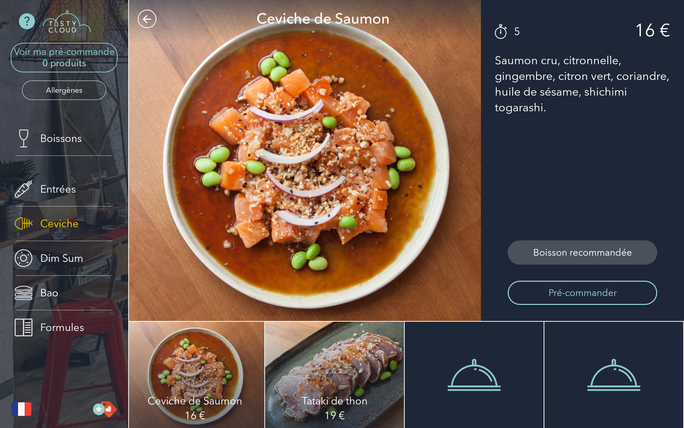
\includegraphics[width=110mm,scale=0.5]{images/couleur_bouton.png}
  \caption{Précédente version graphique}
  \label{fig:boat1}
\end{figure}

On parle ici du bouton "pré-commander" (Figure 3.16), ce dernier présentait auparavant une animation qui le mettait en avant mais celle-ci a dû être retirée. Après concertation sur le basecamp nous avons fait différents choix de couleur qui ont put être discutés en interne avec l'équipe. De toutes ces couleurs je me suis chargé d'en faire des captures d'écran et de les partager. Nous nous sommes concertés sur 2 choix de couleurs précis, le blanc et bleu plein.

\begin{figure}[!htb]
  \centering
  \begin{minipage}[b]{0.45\textwidth}
    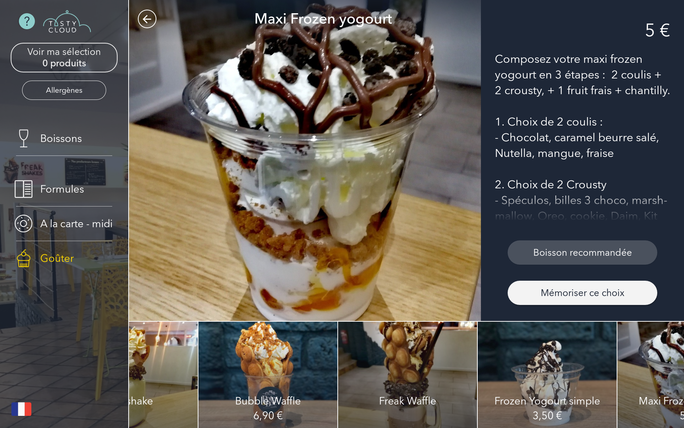
\includegraphics[width=\textwidth]{images/couleur_bouton2.png}
    \caption{Couleur blanche retenu}
  \end{minipage}
  \hfill
  \begin{minipage}[b]{0.45\textwidth}
    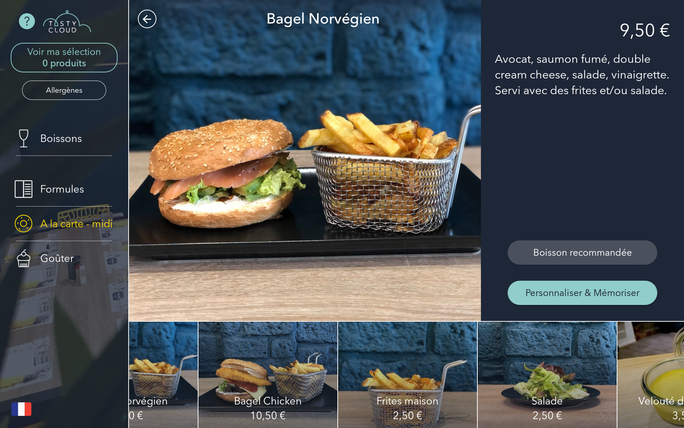
\includegraphics[width=\textwidth]{images/couleur_bouton3.png}
    \caption{Couleur bleu retenu}
  \end{minipage}
\end{figure}

On observe que ce changement affecte aussi le bouton de sélection (voir sa sélection) dans le cas de la couleur blanche. En effet ce dernier a alors des contours blancs. Le problème de cette solution est que l'on a alors 2 couleurs. On a donc décidé de laisser le choix à l'utilisateur (donc ici le restaurateur) de choisir une de ces deux couleurs pour son restaurant. Ce choix s'officie dans le back office où la couleur bleu avec le fond plein est présente par défaut et où la couleur blanche peut être choisie.

Le restaurateur dispose en effet de différentes options cochables ou non comme on peut le voir depuis cette capture d'écran du back office :

\begin{figure}[!htb]
  \centering
  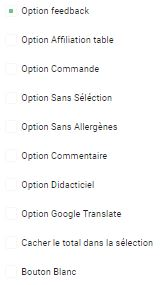
\includegraphics[width=40mm,scale=0.5]{options_backoffice.JPG}
  \caption{Options du back office}
  \label{fig:boat1}
\end{figure}

Pour que cette option fonctionne il a donc fallu rajouter une ligne dans la table "Restaurant" et mettre cela à jour dans les entités dans le code. Avec l'aide de mon tuteur qui avait déjà réalisé des ajouts de fonctionnalités similaires, j'ai pu savoir rapidement les changements à effectuer dans le code. Changer donc l'entité, le modèle (la classe) et le JSON. Tout ceci va nous permettre de faire le lien avec le back office. Il suffit à chaque fois d'ajouter une ligne pour le cas du bouton blanc. 

Une fois ceci terminé on peut récupérer directement avec le restaurant courant la valeur de ce booléen. Il ne faudra alors plus que chercher où mettre cette couleur. En effet elle peut s'appliquer aussi lorsque l'application recommande des plats ou bien lorsque l'on choisit une formule. Une fois tous les cas énumérés ajoutés nous avons pu intégrer cette fonctionnalité dans la version suivante de l'application.

\begin{figure}[!htb]
  \centering
  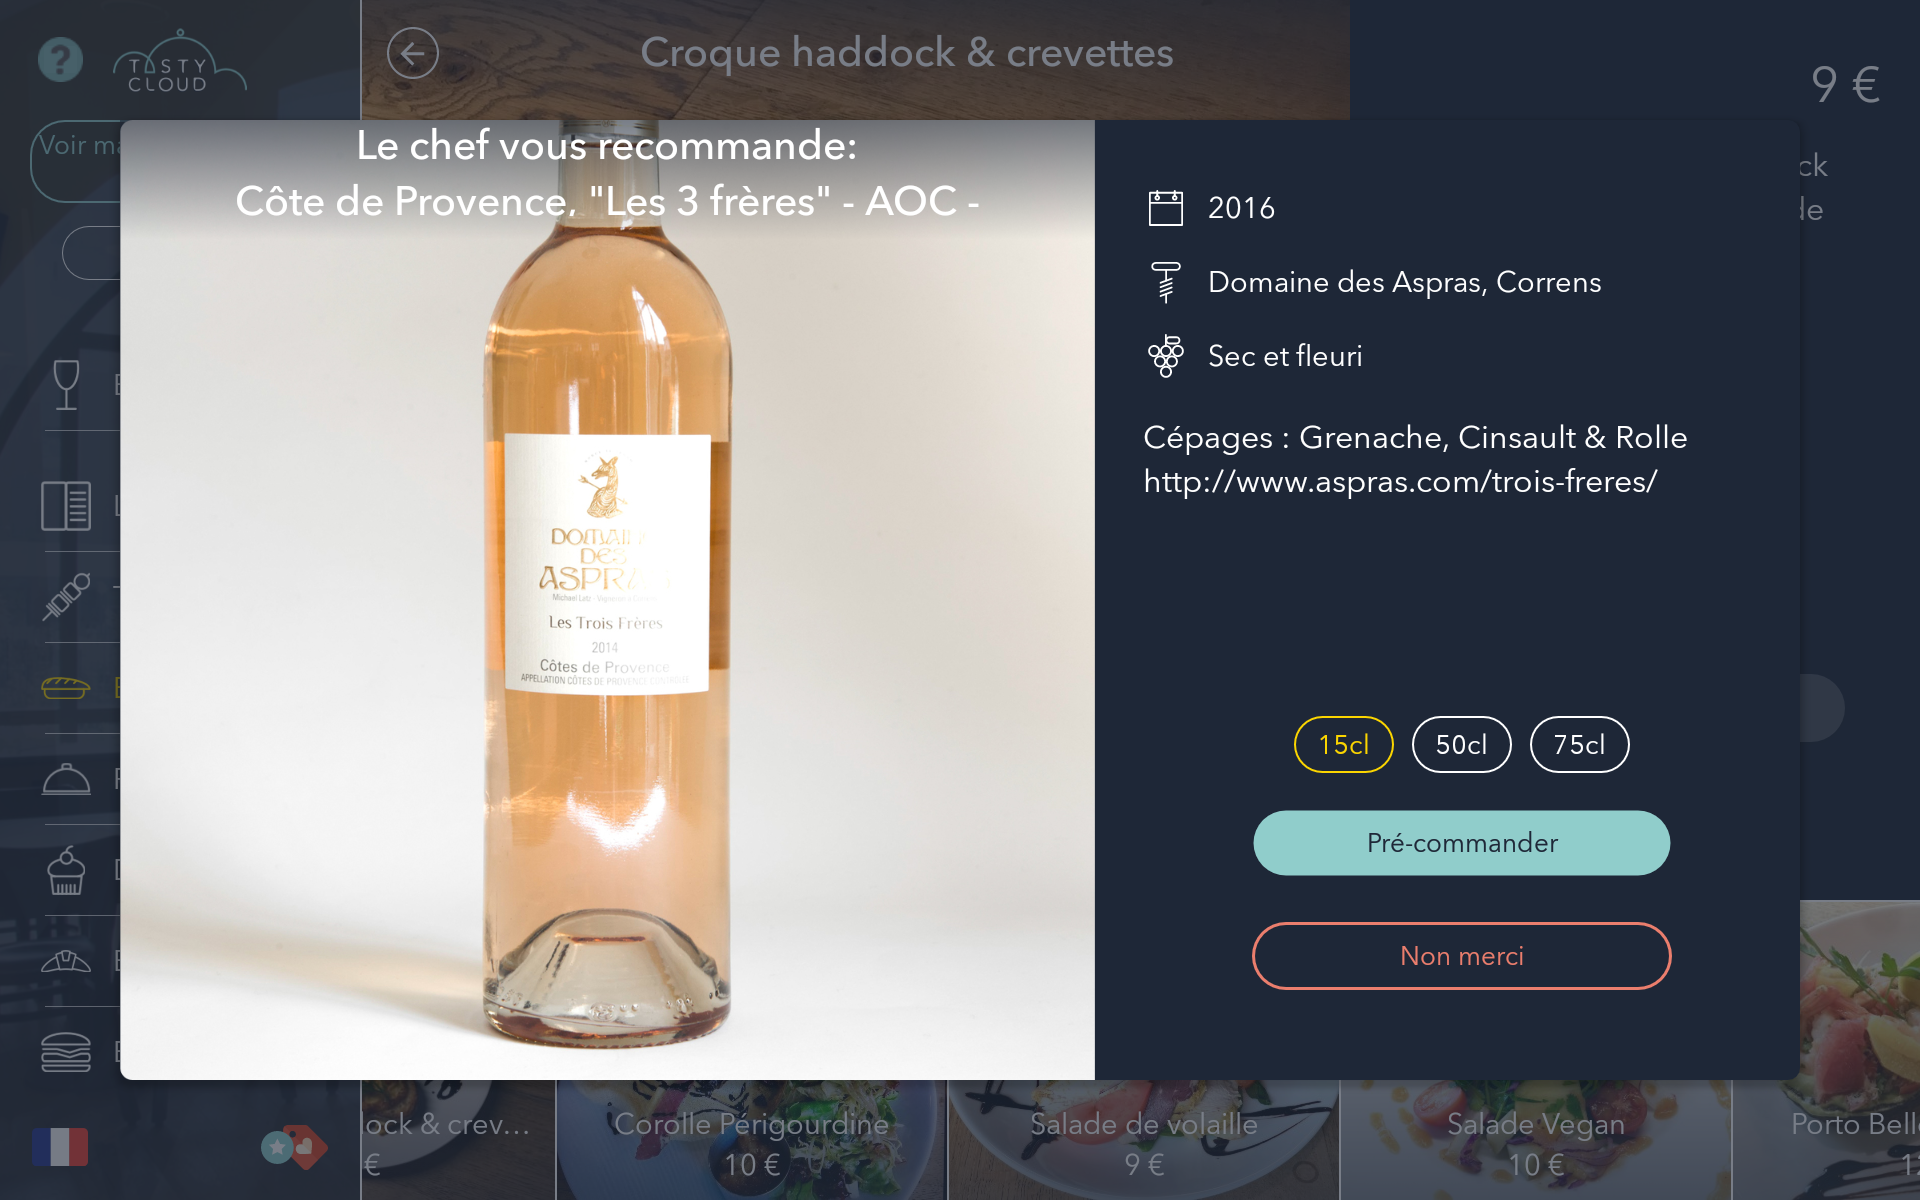
\includegraphics[width=110mm,scale=0.5]{images/couleur_bouton4.png}
  \caption{Une pop-up de recommandation}
  \label{fig:boat1}
\end{figure}

\subsection{Sélection dynamique}

\begin{figure}[!htb]
  \centering
  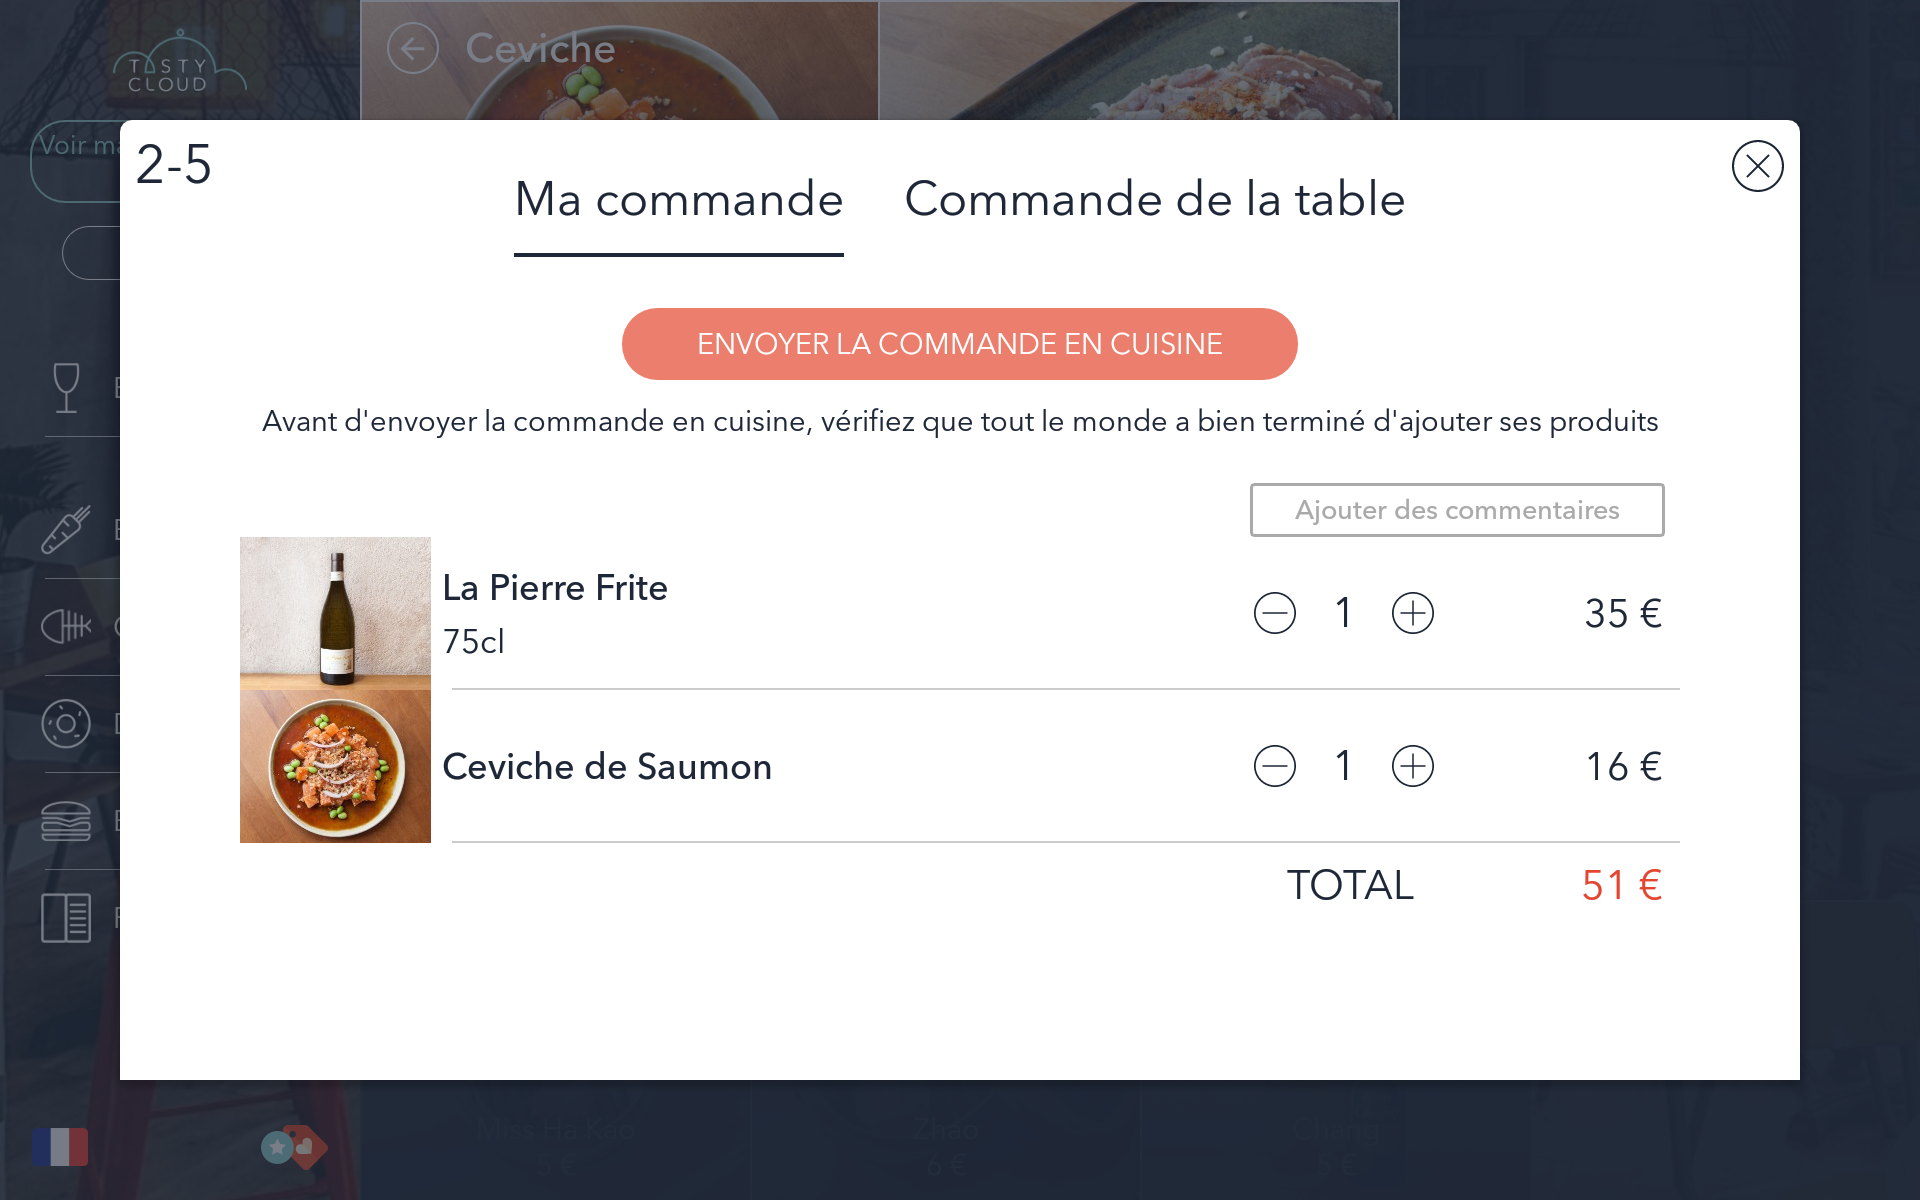
\includegraphics[width=115mm,scale=0.5]{images/selection.png}
  \caption{Menu de sélection}
  \label{fig:boat1}
\end{figure}

Voici le menu de sélection de l'application. Pour certains restaurants, ce menu propose la commande comme dans le cas de la capture d'écran. Il peut aussi être proposé plusieurs tablettes pour une table ce qui fait qu'un utilisateur peut commander sur sa tablette, voir ce qu'il a commandé et aussi voir ce qui a été commandé sur la table dans l'onglet "Commande de la table". L'idée de la mission sur la sélection dynamique est que cet onglet apparaît si et seulement si quelqu'un d'autre a commandé quelque chose. On peut donc aussi avoir le cas ou "Ma commande" est vide et "Commande de la table" est présent. Tout dépend la manière dont les plats sont commandés. Le but de cette mission était aussi que tout cela se fasse en temps réel. Pour ce faire mon tuteur m'a expliqué que je devais passer par le presenter et faire cela de manière asynchrone comme ce qui a par exemple été fait pour l'affiliation. Dans le contrôleur j'ai donc une fonction de ce type :

\begin{lstlisting}[frame=single]  % Start your code-block
    
    override fun bindTablesEachOther(isDifferent: Boolean) {
        if(isDifferent)
            tab2.visible()
        else
            tab2.gone()
    }
    
\end{lstlisting}

Elle permet simplement de cacher oui ou non le deuxième onglet, si les deux listes sont différentes. Pour ce qui est du paramètre passer à la fonction, c'est via le presenter qu'il est appelé. On va récupérer les deux listes depuis la base de données et faire les tests nécessaires pour savoir si oui ou non elles sont différentes. J'ai, dans un premier temps, fait simplement un test sur la taille des deux listes et retourner vrai si différent. Cependant, les listes sont différentes si le nombre de choix pour un produit change. Par exemple, il est possible que l'on ait la même taille dans la liste (par exemple 2 sur la figure 3.21) mais que dans la commande de la table l'on ait 2 ceviche de saumon et 1 vin "La Pierre Frite". Les listes auront bien la même taille mais le nombre de produits réels sera 2 chez moi et 3 sur la commande de la table.

\clearpage

Pour résoudre ce problème il a fallu faire plus de test. Nous avons le test des tailles il faut aussi tester les items un par un dans un foreach. Pour chacun on test si le nombre d'éléments est différent (1 vin ? 2 vin ?) et on test si c'est bien les mêmes produits. Si dans les deux cas il y a une différence alors on retournera vrai. Après avoir implémenté cette solution j'ai pu tester avec deux tablettes en même temps sur une table. Cela semblait bien fonctionner mais j'ai ensuite remarqué que les produits n'étaient pas rangés de la même façon selon que l'on soit dans le premier ou deuxième onglet.

\begin{figure}[!htb]
  \centering
  \begin{minipage}[b]{0.45\textwidth}
    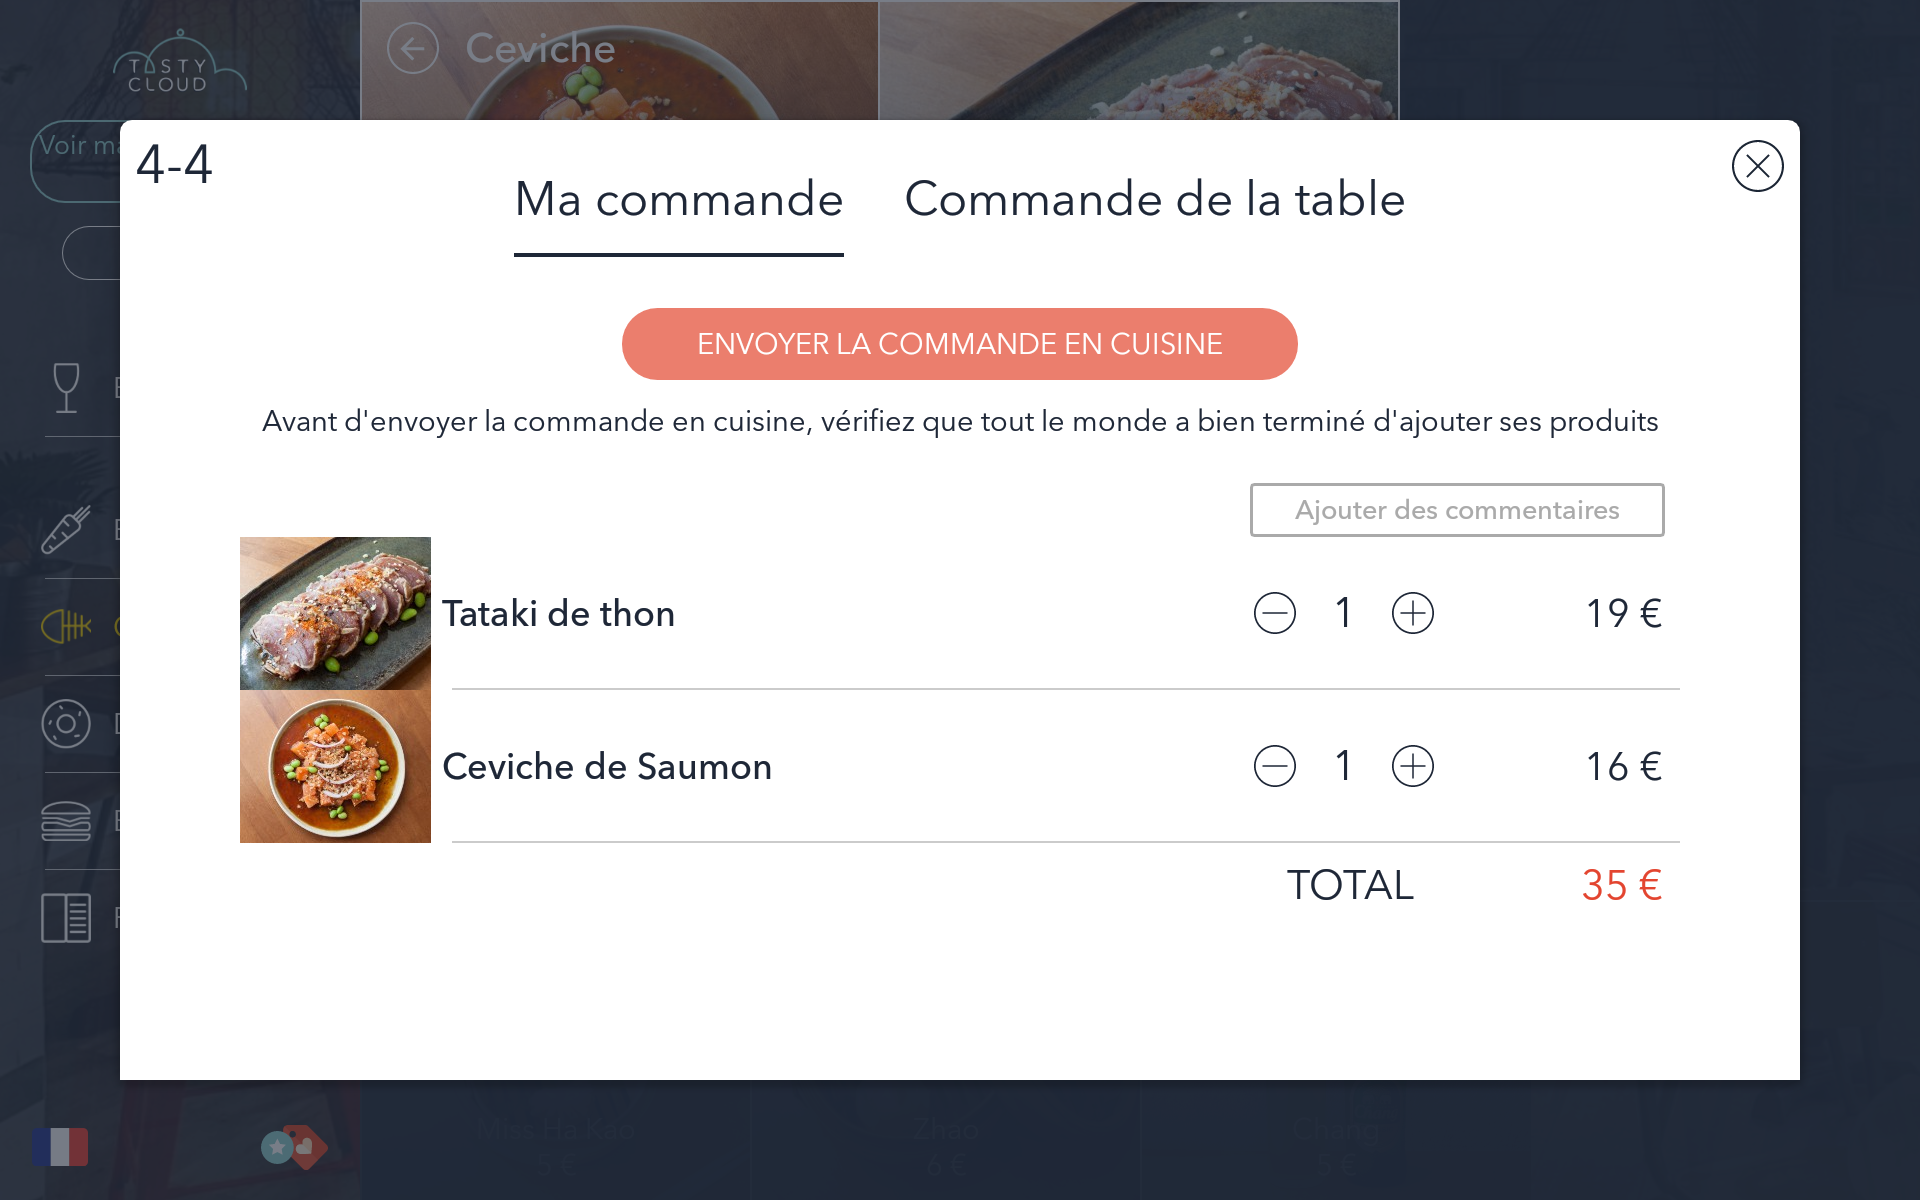
\includegraphics[width=\textwidth]{images/selection2.png}
    \caption{Onglet "Ma commande"}
  \end{minipage}
  \hfill
  \begin{minipage}[b]{0.45\textwidth}
    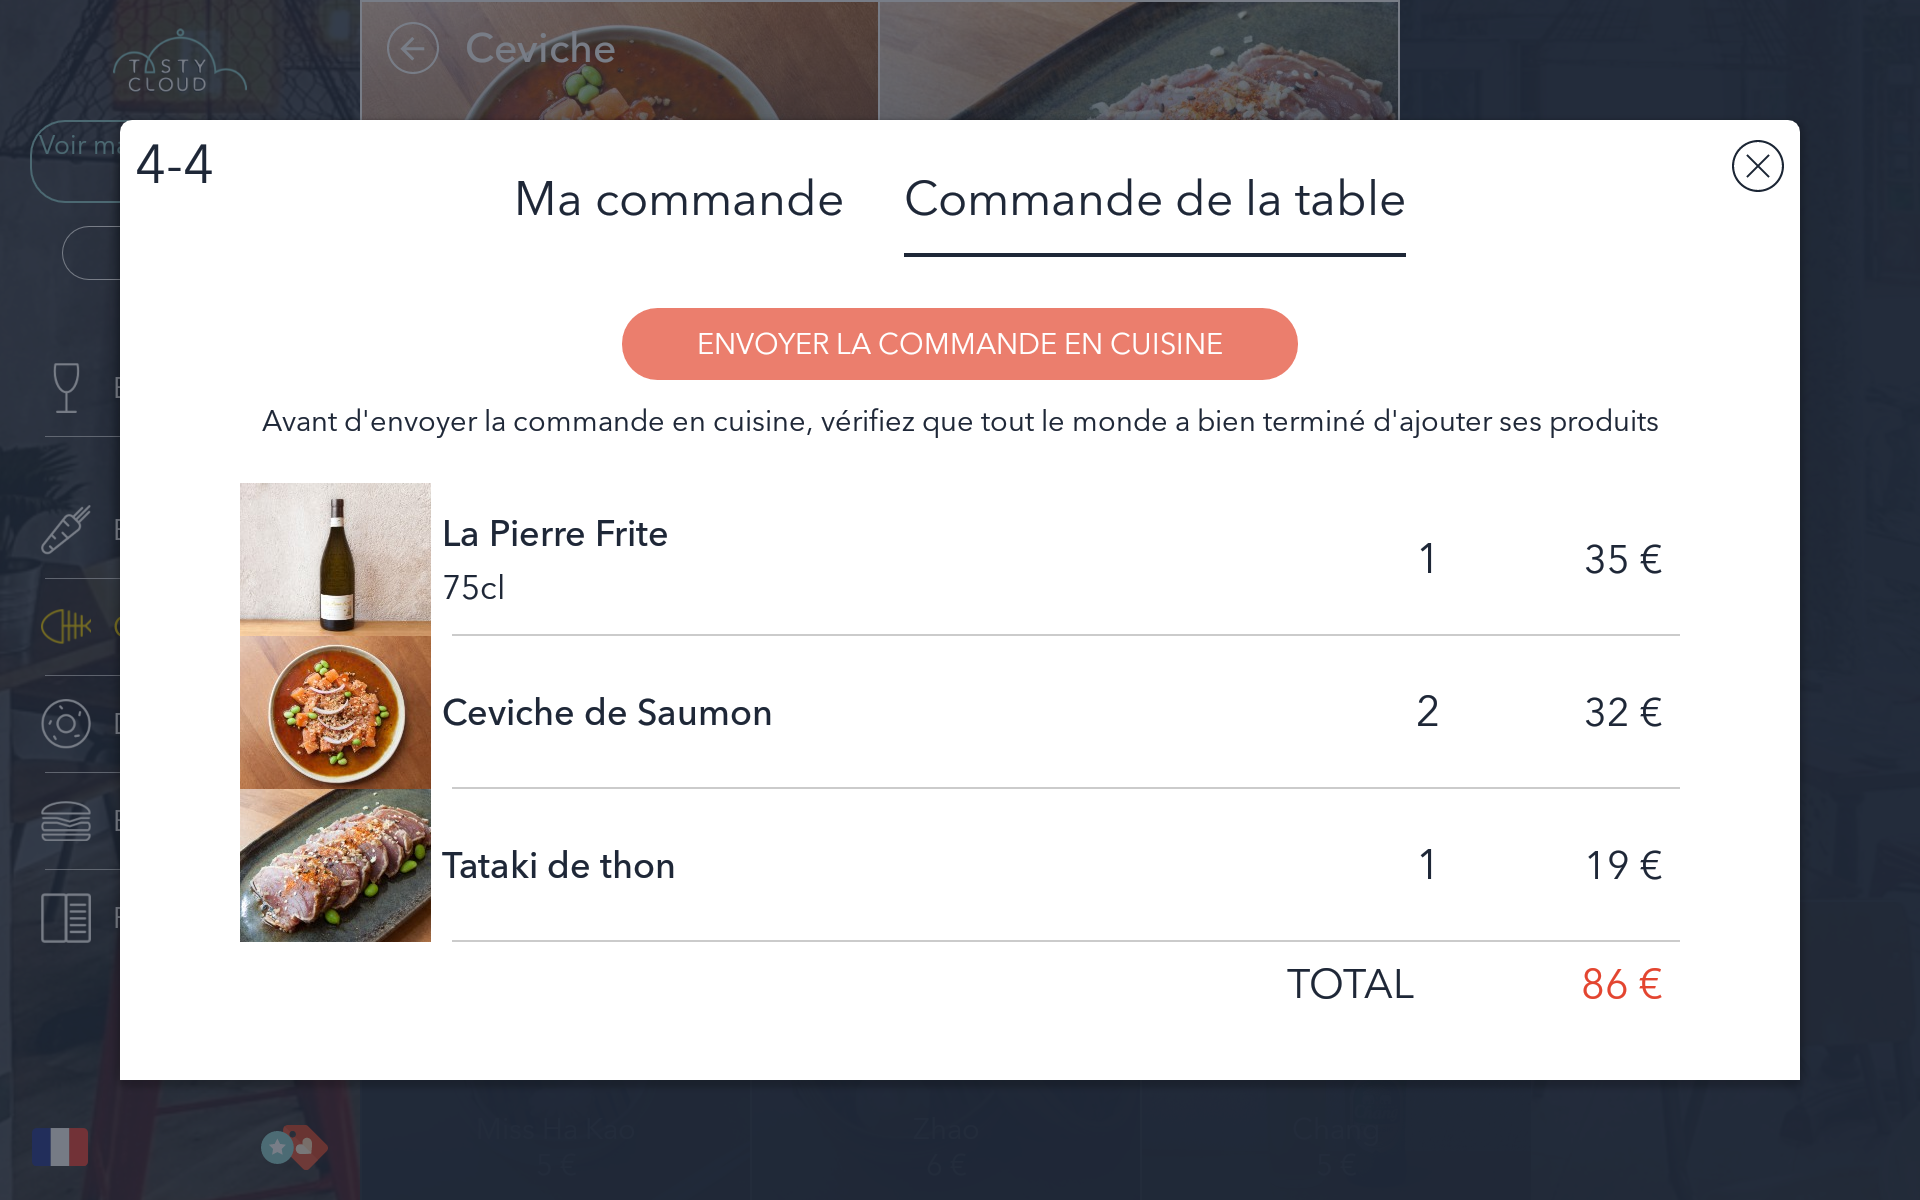
\includegraphics[width=\textwidth]{images/selection3.png}
    \caption{Onglet "Commande de la table"}
  \end{minipage}
\end{figure}

Par exemple dans ma commande, on a "Tataki de thon" puis "Ceviche de saumon" et ces deux aliments sont inversés dans commande de la table. Ceci s'explique que pour des raisons pratiques de traitements, les aliments dans commande de la table doivent être triés de façon précise (par les id des produits) et dans ma commande, ils doivent l'être dans l'ordre dans lesquels les produits ont été commandés. En conséquence de cela, il a fallu repenser le système de comparaison et c'est alors que j'ai décidé  de faire l'addition de tous les nombres de produits et de les comparer. Par exemple dans les deux captures d'écran ci-dessus, on aurait 2 à gauche et 4 à droite et donc l'affichage de l'onglet "Commande de la table".

Ainsi cette mission est pratique pour le visuel des clients en salle. Ils peuvent tout de suite connaître et voir en temps réel les ajouts et suppressions des convives avec lesquels ils sont. Lors de la visualisation de leur commande, ils peuvent voir si l'onglet "Commande de la table" apparaît ou non et ainsi constater si il y déjà eu une commande à leur table.

\begin{figure}[!htb]
  \centering
  \begin{minipage}[b]{0.45\textwidth}
    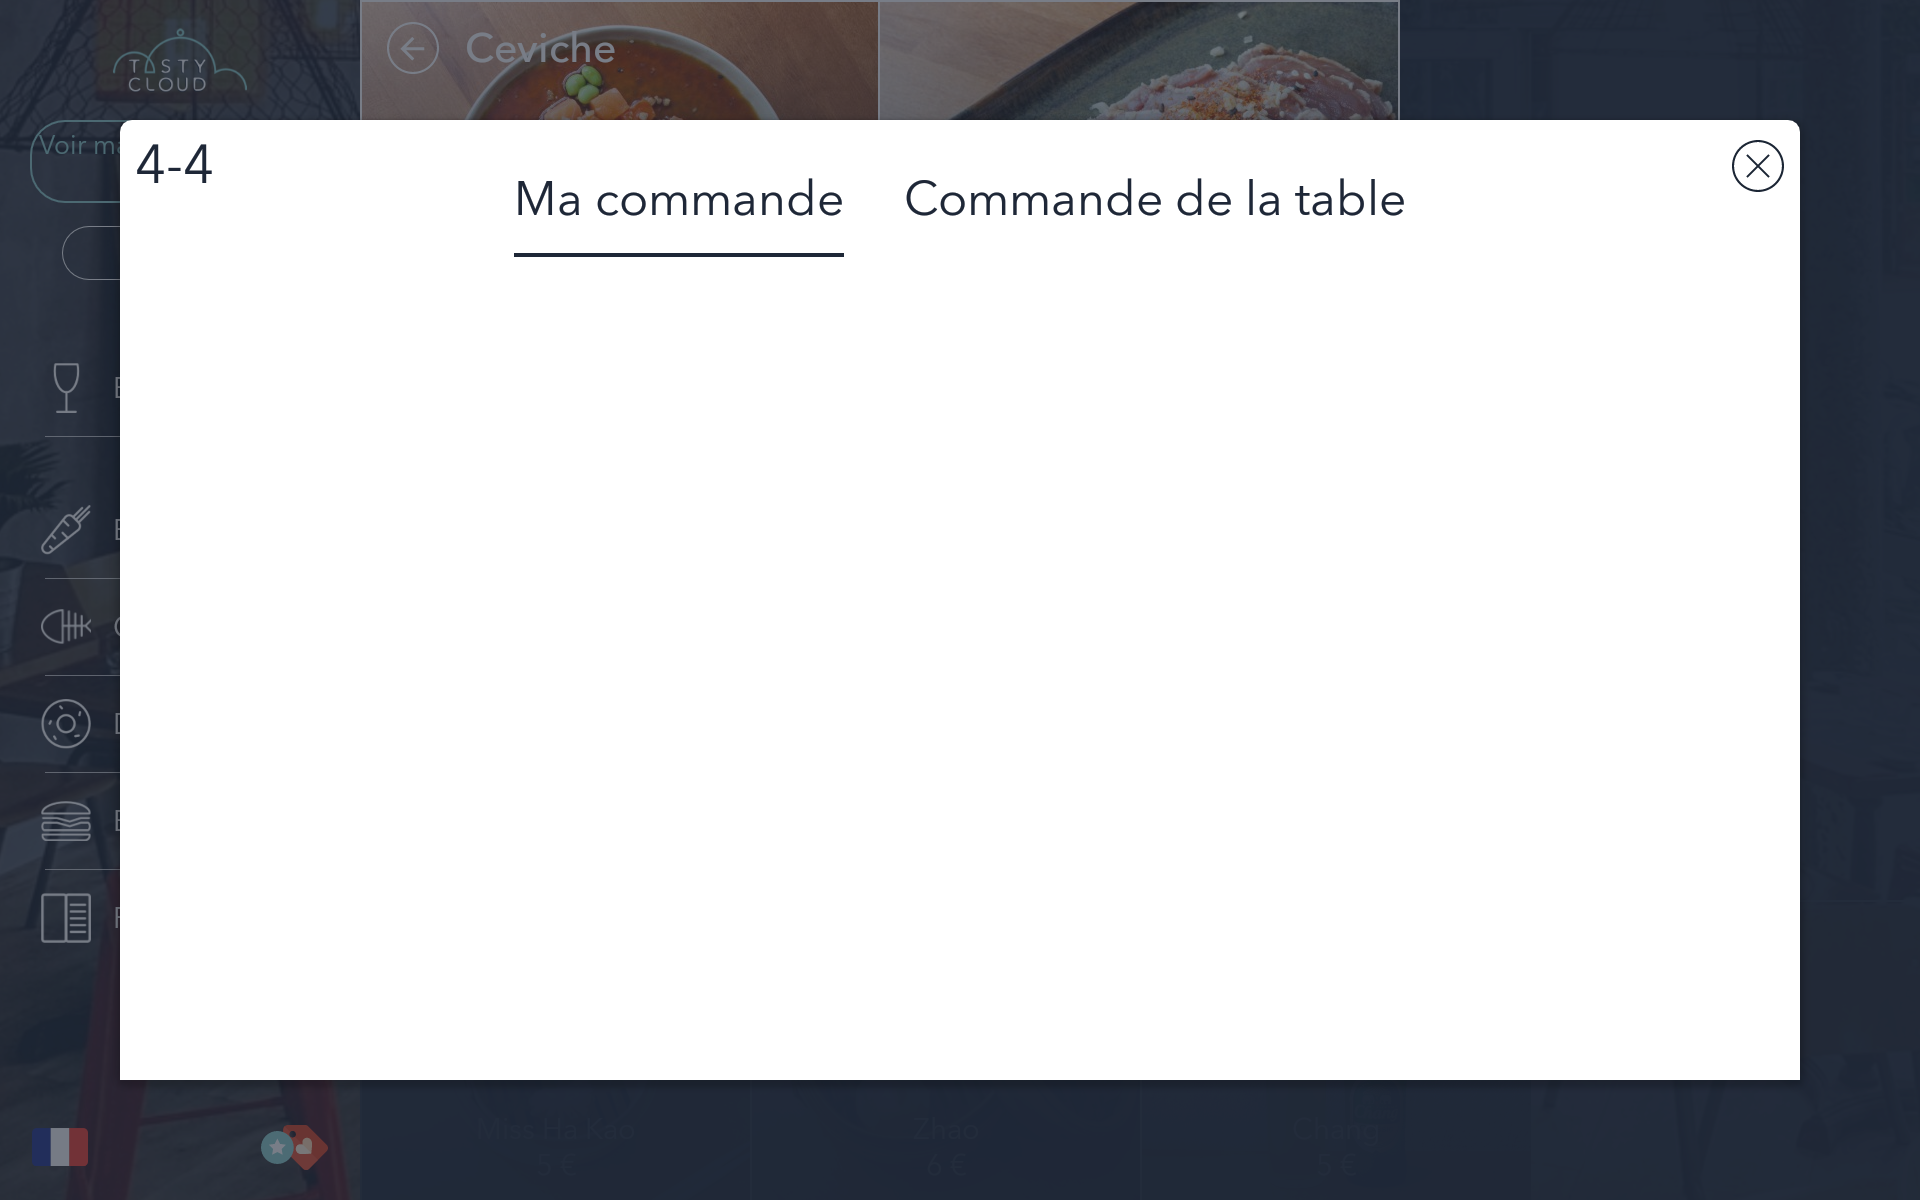
\includegraphics[width=\textwidth]{images/selection4.png}
    \caption{Cas ou quelqu'un a commandé}
  \end{minipage}
  \hfill
  \begin{minipage}[b]{0.45\textwidth}
    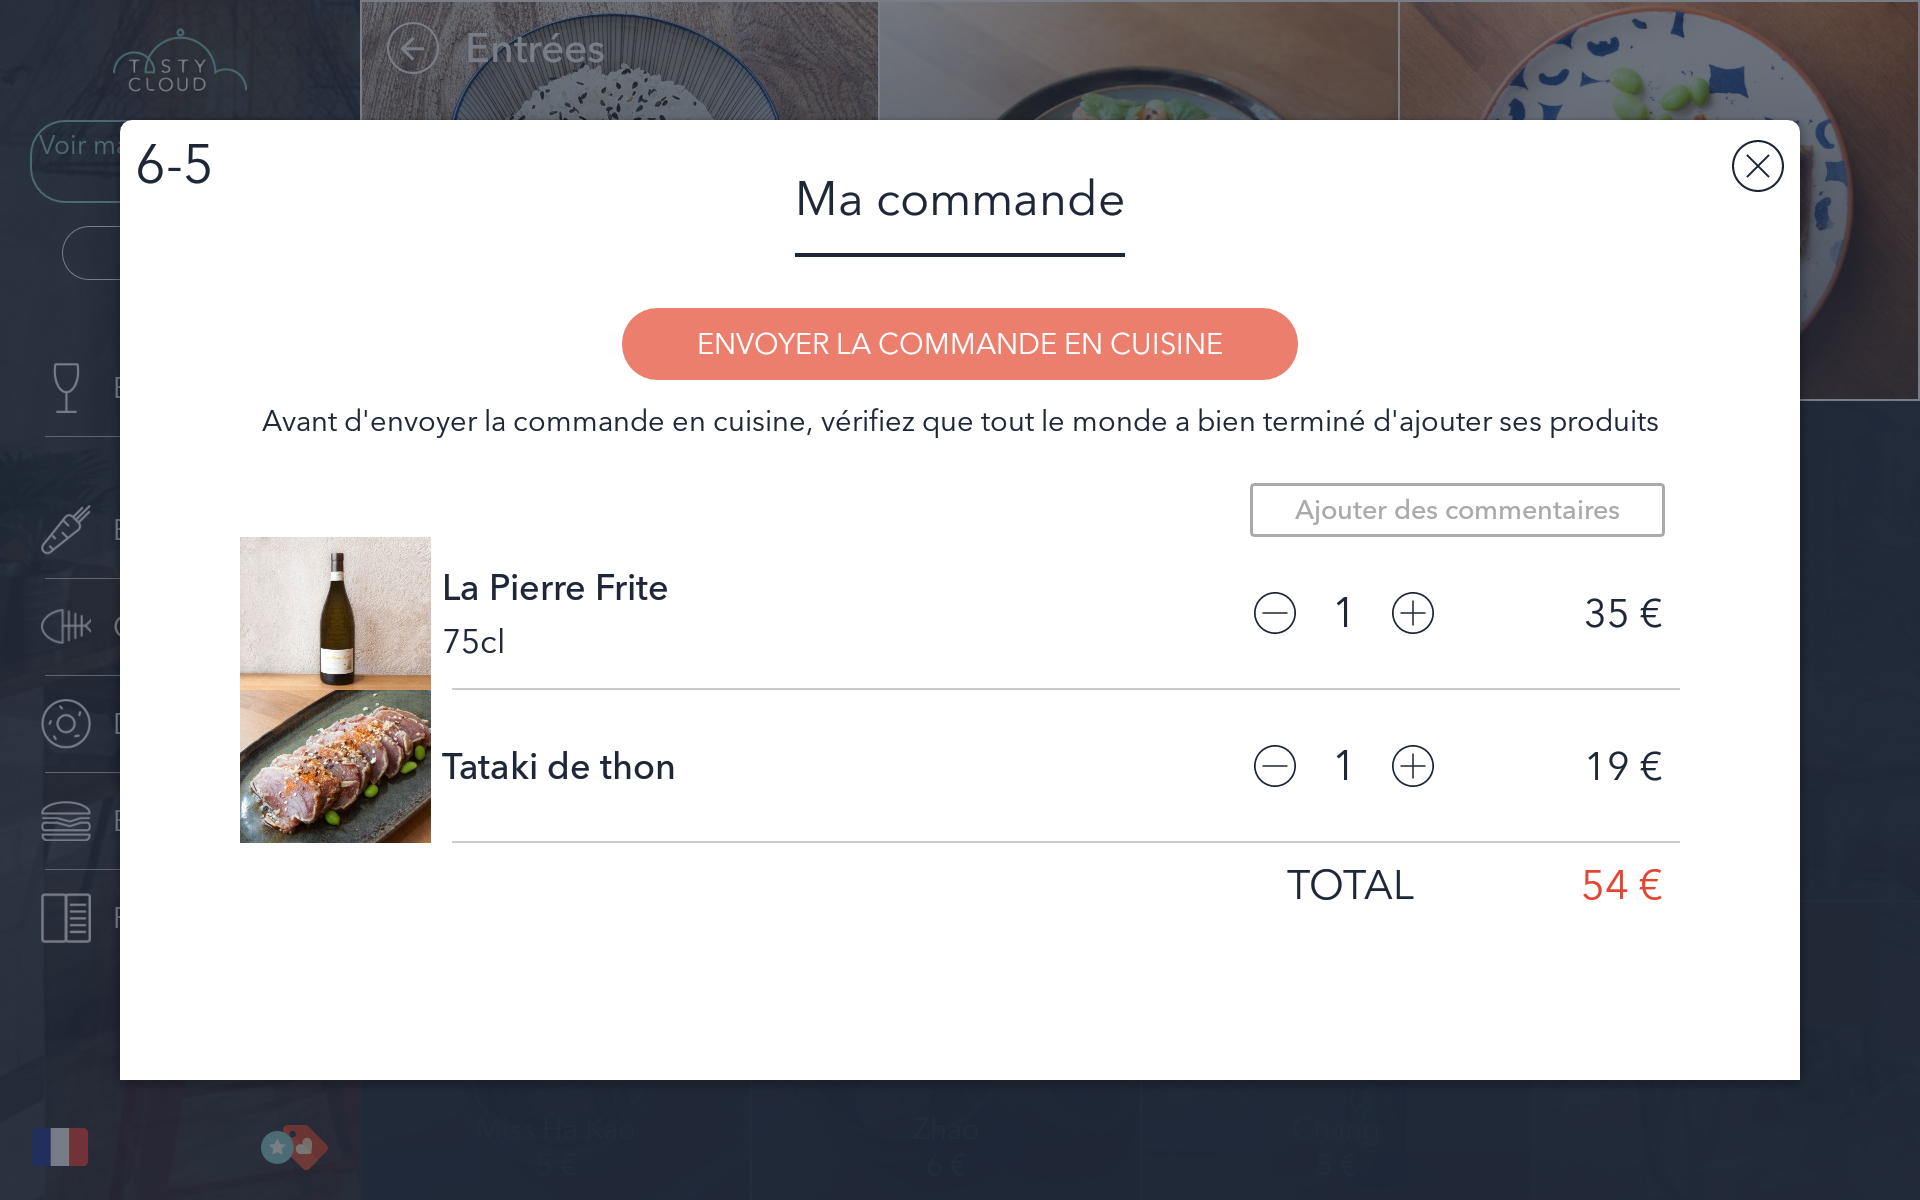
\includegraphics[width=\textwidth]{images/selection5.png}
    \caption{Cas ou je suis le seul à avoir commandé}
  \end{minipage}
\end{figure}



\subsection{Mot de passe pour la clôture de tables}

Certains serveurs mal informés appuyaient inopinément sur le bouton "Clôturer service". Ce bouton ferme toutes les tables du restaurant sans préavis. Avec mon tuteur, nous avons donc pensé à créer une boite de dialogue qui s'ouvre quand on appuie sur ce bouton. Cette dernière demande alors un mot de passe qui permet de clôturer toutes les tables et ainsi l'erreur n'est plus possible. Pour cette mission il n'y pas vraiment de modélisation ou de conception à réaliser. Seulement, nous nous sommes rendus compte que le DialogBox précédemment énoncé dans le rapport ne s'affichait pas sur la page d'affiliation. On a réutilisé alors PopupWindow qui lui se plaçait en premier plan sur l'affiliation (qui est aussi techniquement une pop-up). Il a alors fallu faire un XML correspondant à ce qui était requis pour la demande de clôture de tables soit un champ d'édition de texte pour le mot de passe et deux boutons "Valider" et "Fermer".

\begin{figure}[!htb]
  \centering
  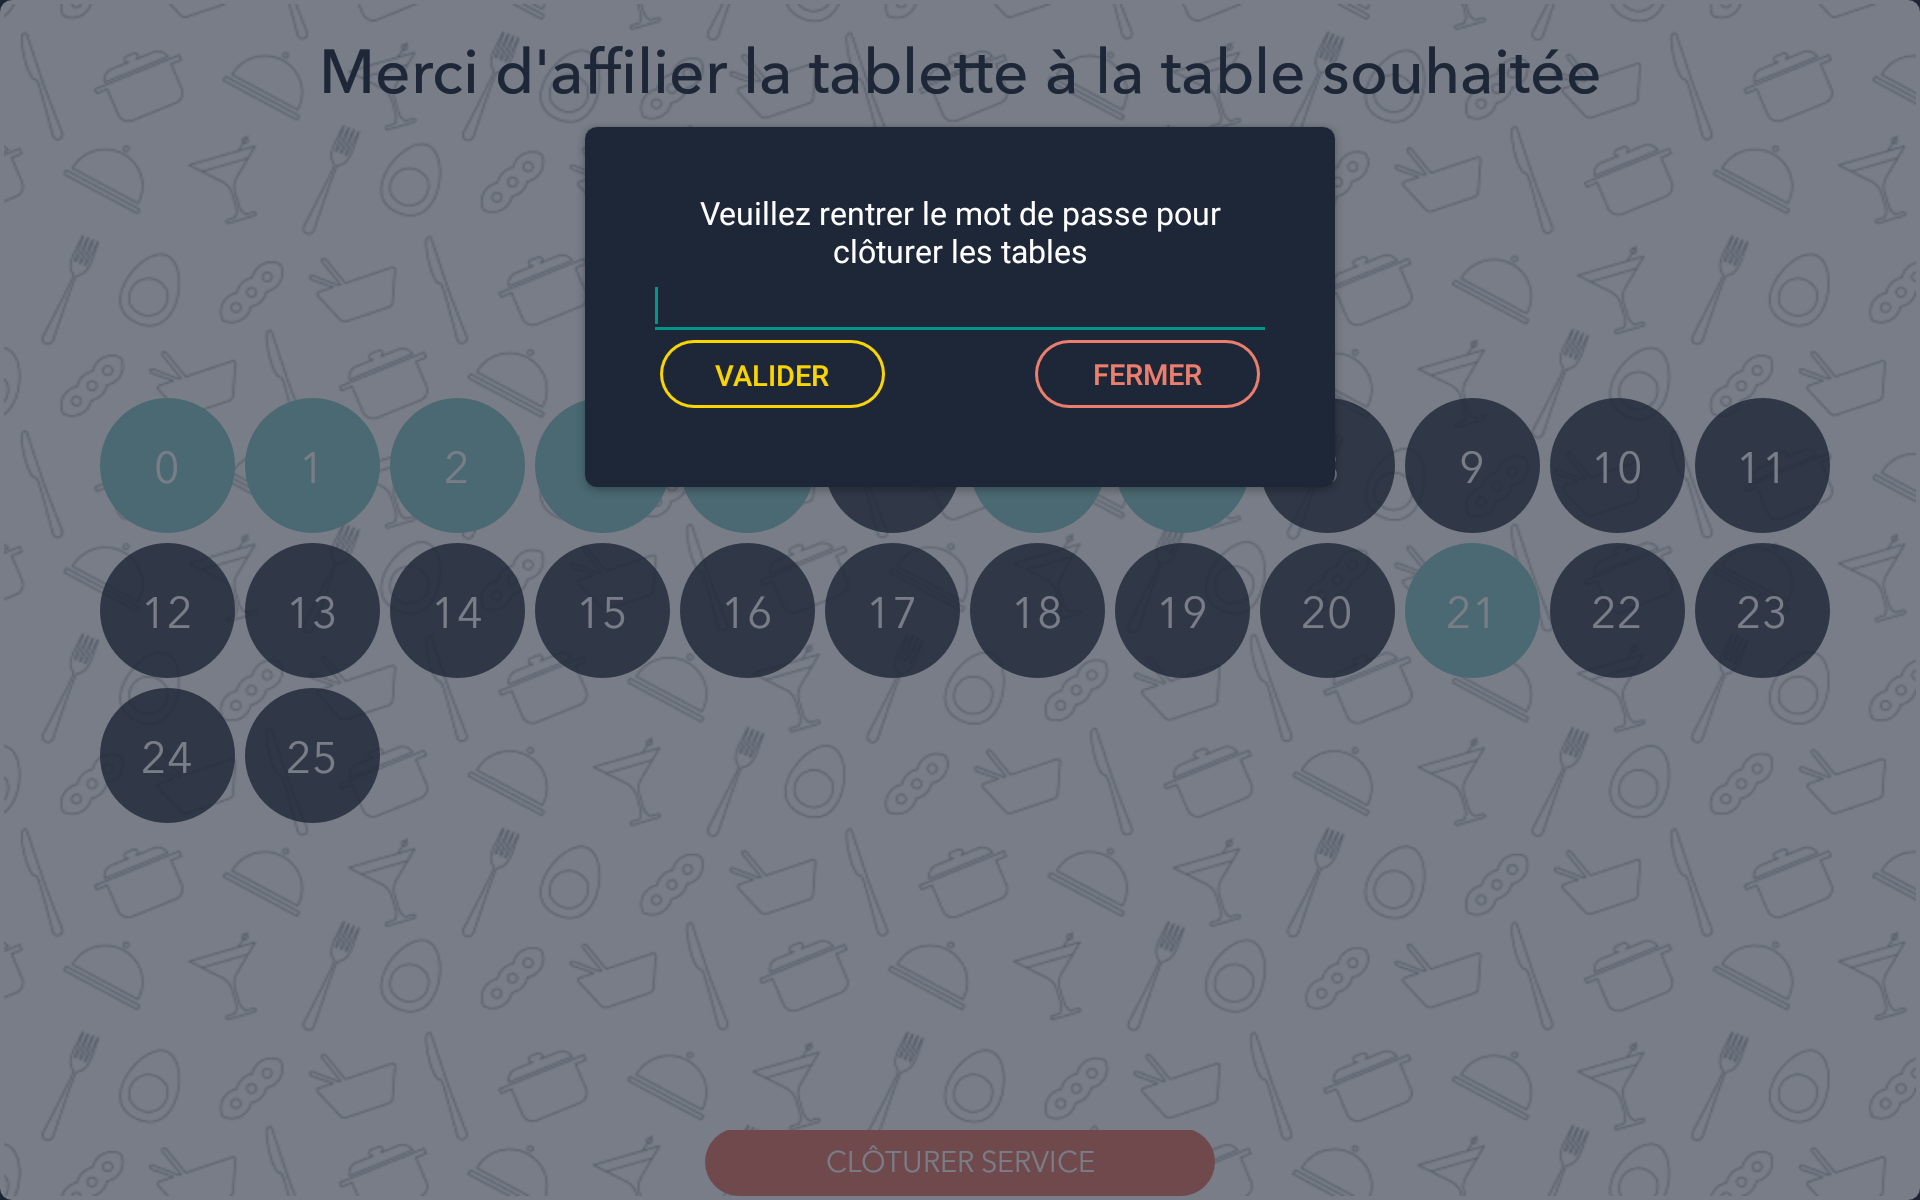
\includegraphics[width=100mm,scale=0.5]{images/cloture_table.png}
  \caption{Fenêtre pour la fermeture des tables}
  \label{fig:boat1}
\end{figure}

Le mot de passe demandé est toujours le même.Nous avons alors respecté la charte graphique qui existait déjà sur certaines autres pop-ups. Le but de cette mission était de sécuriser l'application pour la clôture de table. Fermer toutes les tables alors que l'on est en plein service peut s'avérer très dangereux.

\begin{figure}[!htb]
  \centering
  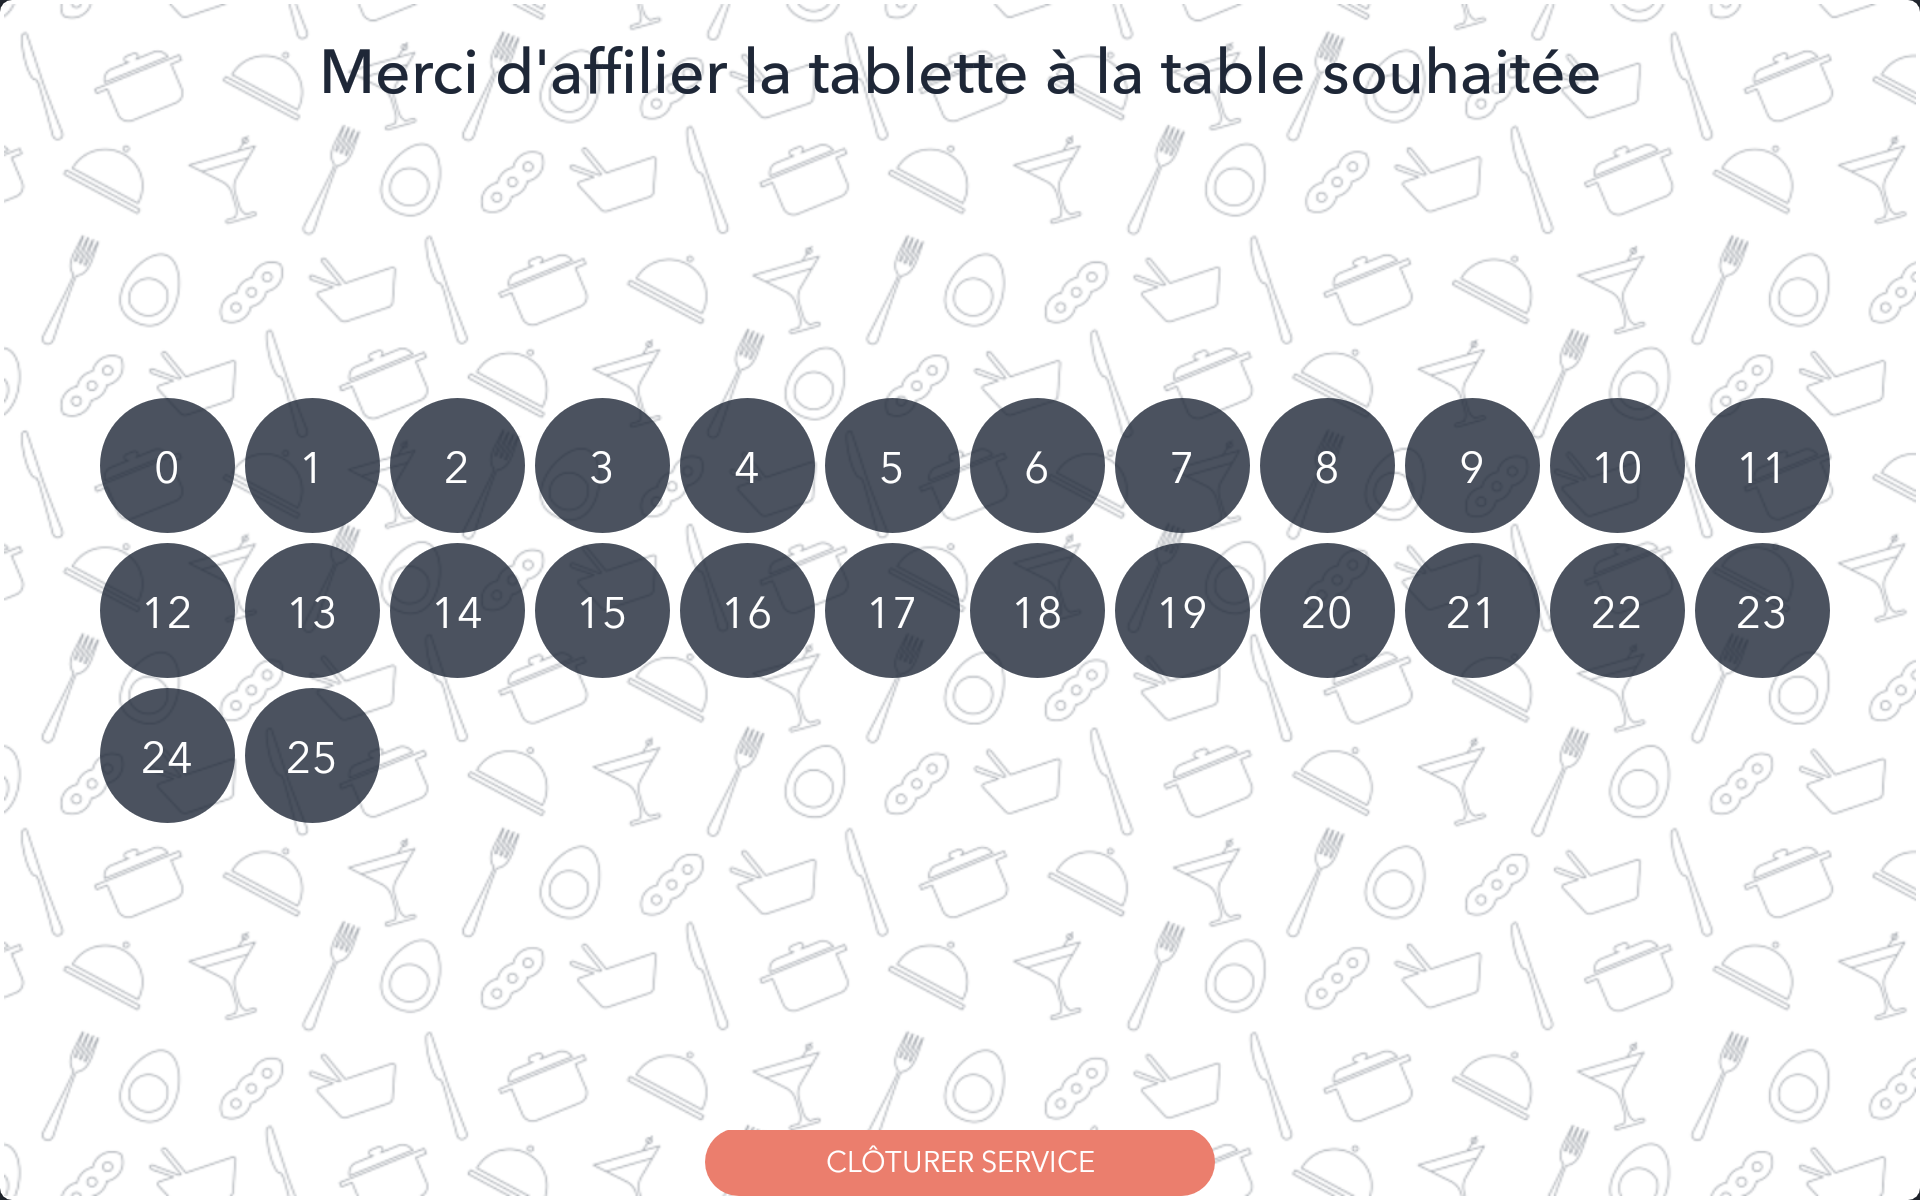
\includegraphics[width=100mm,scale=0.5]{images/cloture_table2.png}
  \caption{Toutes les tables sont fermés !}
  \label{fig:boat1}
\end{figure}


\subsection{Les descriptions scrollable visibles}

Certains produits possèdent des descriptions longues et dans certains cas l'aménagement du texte fait que l'on n'a pas forcément l'information que l'on peut scroller (ou dérouler) pour voir la suite.

\begin{figure}[!htb]
  \centering
  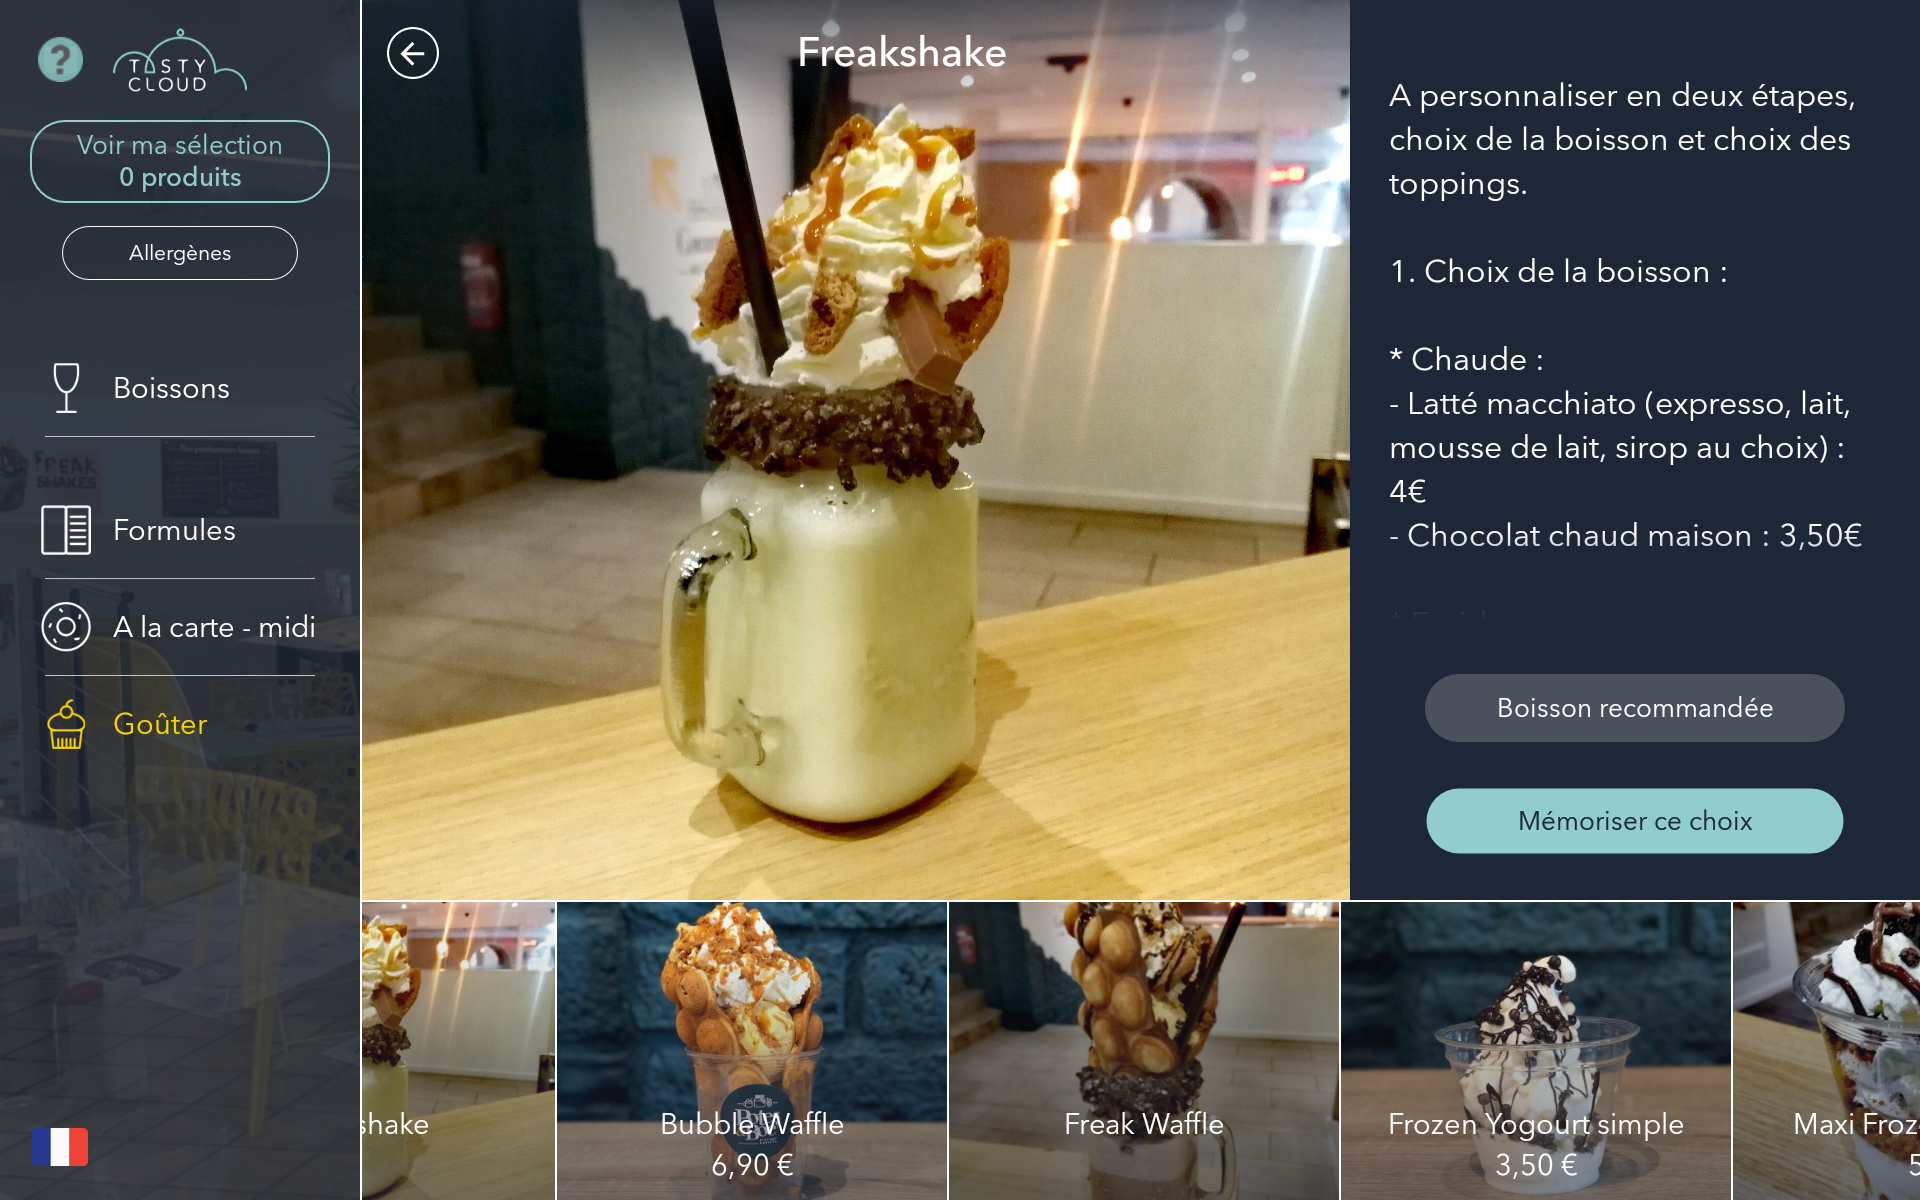
\includegraphics[width=100mm,scale=0.5]{images/scroll.png}
  \caption{Il est ici pas évident de savoir si on peut scroller}
  \label{fig:boat1}
\end{figure}

Voici par exemple un cas où le bas de la description coïncide avec un saut à la ligne. Ici le client peut passer à côté de ce qu'il y a écrit en dessous. Pour ce cas précis il s'agit d'expliquer une formule. Par conséquent il m'a été chargé de trouver un moyen pour régler ce problème. Ma première approche a été de changer la taille de la décoloration des bords pour que l'on voit mieux qu'il est possible de scroller vers le bas. Seulement, l'attribut à changer en XML fait que cela change le bas et le haut. J'ai alors fait en sorte que le bas du rectangle de description coïncide toujours avec une ligne de texte pour que cette dernière soit coupée. Ici le problème est que ce rectangle peut changer de taille. En effet pour les vins par exemple nous avons la provenance la date, ses caractéristiques qui prennent le haut droit de la page (au-dessus de la description). Par conséquent il est assez difficile de prévoir tous les cas possibles. 

J'ai donc abandonné cette idée pour finalement me rabattre sur la première mais cette fois en essayant de trouver une solution pour changer la décoloration juste en bas. En m'intéressant à la classe "ScrollView" d'Android (donc la classe qui nous permet de scroller), je me suis rendu compte que cette classe contenait deux fonctions "getTopFadingEdgeStrength" et "getBottomFadingEdgeStrength". Si le haut ne pose pas de problème il faut accentuer l'effet de décoloration du scrollview en bas. J'ai décidé de laisser le fonctionnement du "getBottomFadingEdgeStrength" comme il était mais de changer le top. Je voulais en effet limiter cette accentuation sur le top. Ainsi je pourrais utiliser l'attribut "FadingEgeLength" dans le XML en le mettant à un pourcentage élevé. Le top lui sera affecté à 20 pourcent de cette valeur avec la redéfinition de la fonction.

L'idée était donc de créer une classe qui étend de ScrollView et de redéfinir son "getTopFadingEdgeStrength" pour que ce dernier retourne 20 pourcents de la valeur qu'on lui a attribué dans le XML (le code de cette fonction est disponible en annexe). On utilisera alors cette classe comme ScrollView dans le XML.

\clearpage

\begin{figure}[!htb]
  \centering
  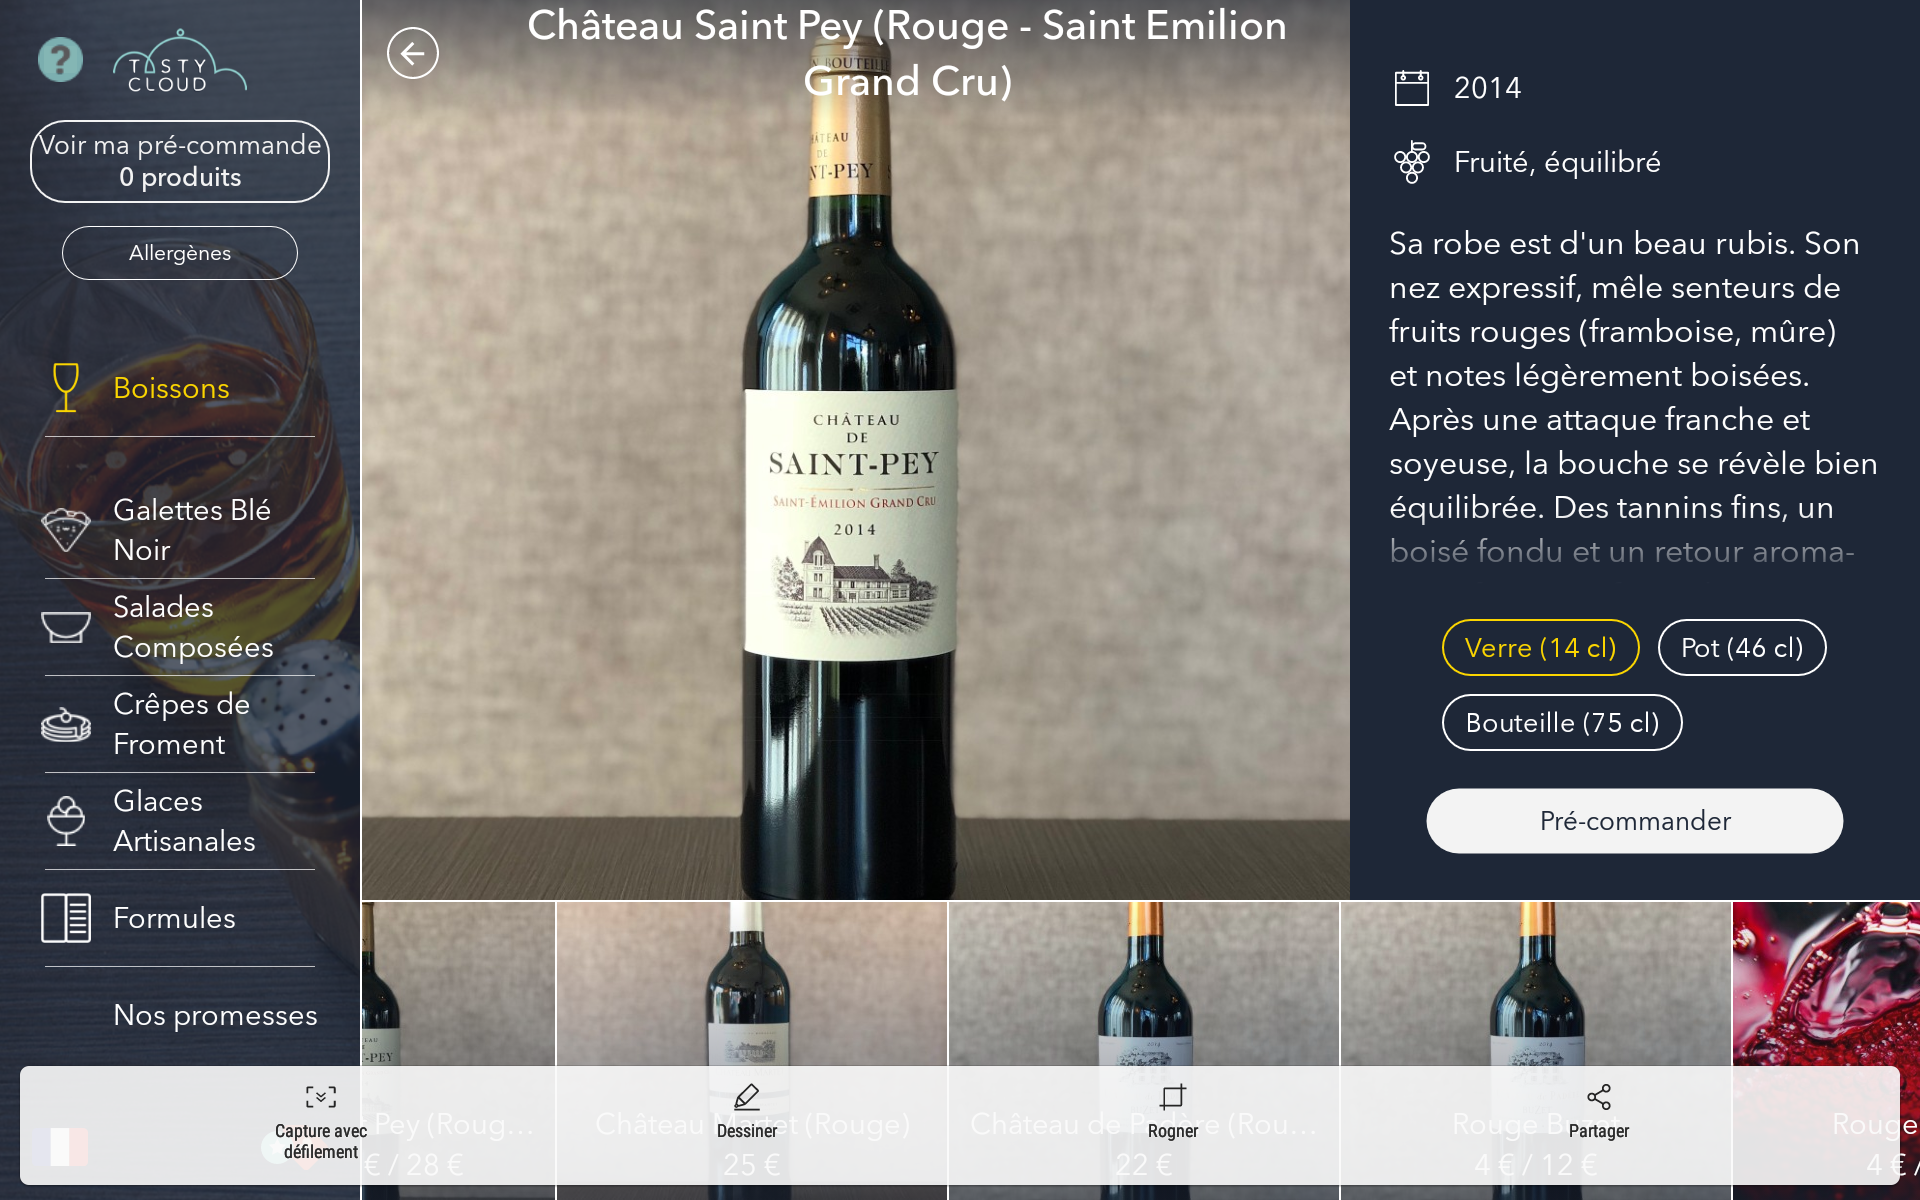
\includegraphics[width=115mm,scale=0.5]{images/scroll2.png}
  \caption{Effet de décoloration sur la description}
  \label{fig:boat1}
\end{figure}

On peut voir un exemple de cette décoloration sur la figure ci-dessus. J'en profite aussi pour montrer les caractéristiques présentes sur les vins par rapport à ce qui a été dit précédemment. On a par exemple ici la date et les caractéristiques du vin qui compressent la description. Pour la deuxième solution il était difficile de la mettre en place car il y avait trop de cas différents.

Par rapport à la décoloration, on voit bien ici que la description est scrollable. Prenons un autre cas où l'on voit bien la différence de taille entre le bas et le haut.

\begin{figure}[!htb]
  \centering
  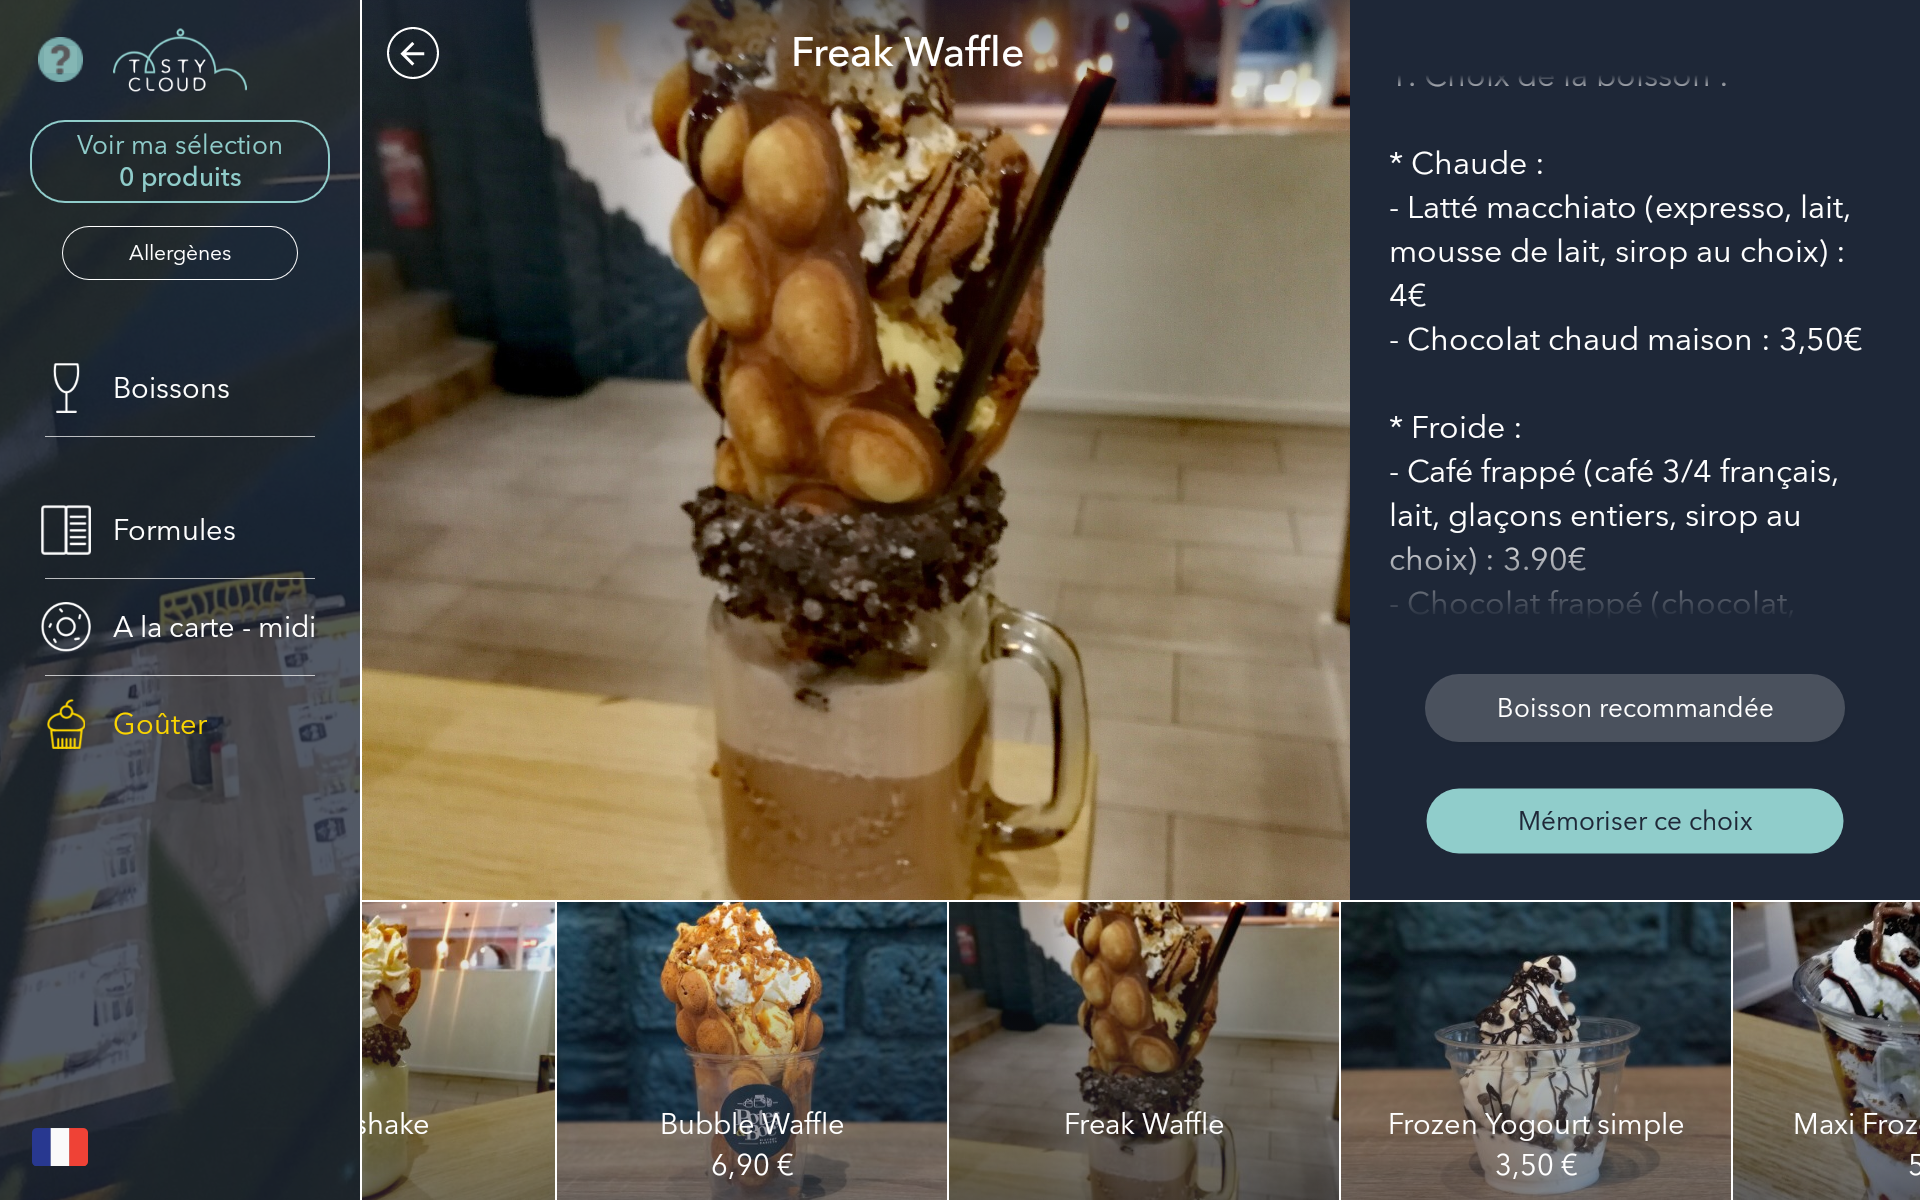
\includegraphics[width=115mm,scale=0.5]{images/scroll3.png}
  \caption{Différence décoloration haut et bas}
  \label{fig:boat1}
\end{figure}

Si dorénavant le bas de la description coïncide avec un retour à la ligne ou même un saut de ligne, l'utilisateur pourra constater le dégradé qui lui suggérera alors de dérouler la description. Cette mission peut paraître anodine mais elle tout de même importante pour accentuer la stabilité de l'application et montrer qu'il y a eu un gros travail sur le feedback client pour proposer la meilleure expérience possible aux utilisateurs.

\section{Divers}

Dans cette partie, je vais présenter différentes missions réalisées durant le stage qui sont soit minimes soit comparables à d'autres missions déjà présentées. Je vais aussi parler de choses pas directement en rapport avec ma mission de stage (donc le développement android).

Comme pour la mission du bouton blanc, une autre demande client était de cacher le total dans le menu de sélection où l'on voit ses plats choisis. Comme seulement quelques restaurants en particulier voulaient cette fonctionnalité, on a fait une option dans le back office. Il a donc juste fallu cacher le total dans le cas où la case correspondante à cette option était cochée. Voici un exemple où le total est caché, il n'est plus affiché en dessous de la liste des produits.

\begin{figure}[!htb]
  \centering
  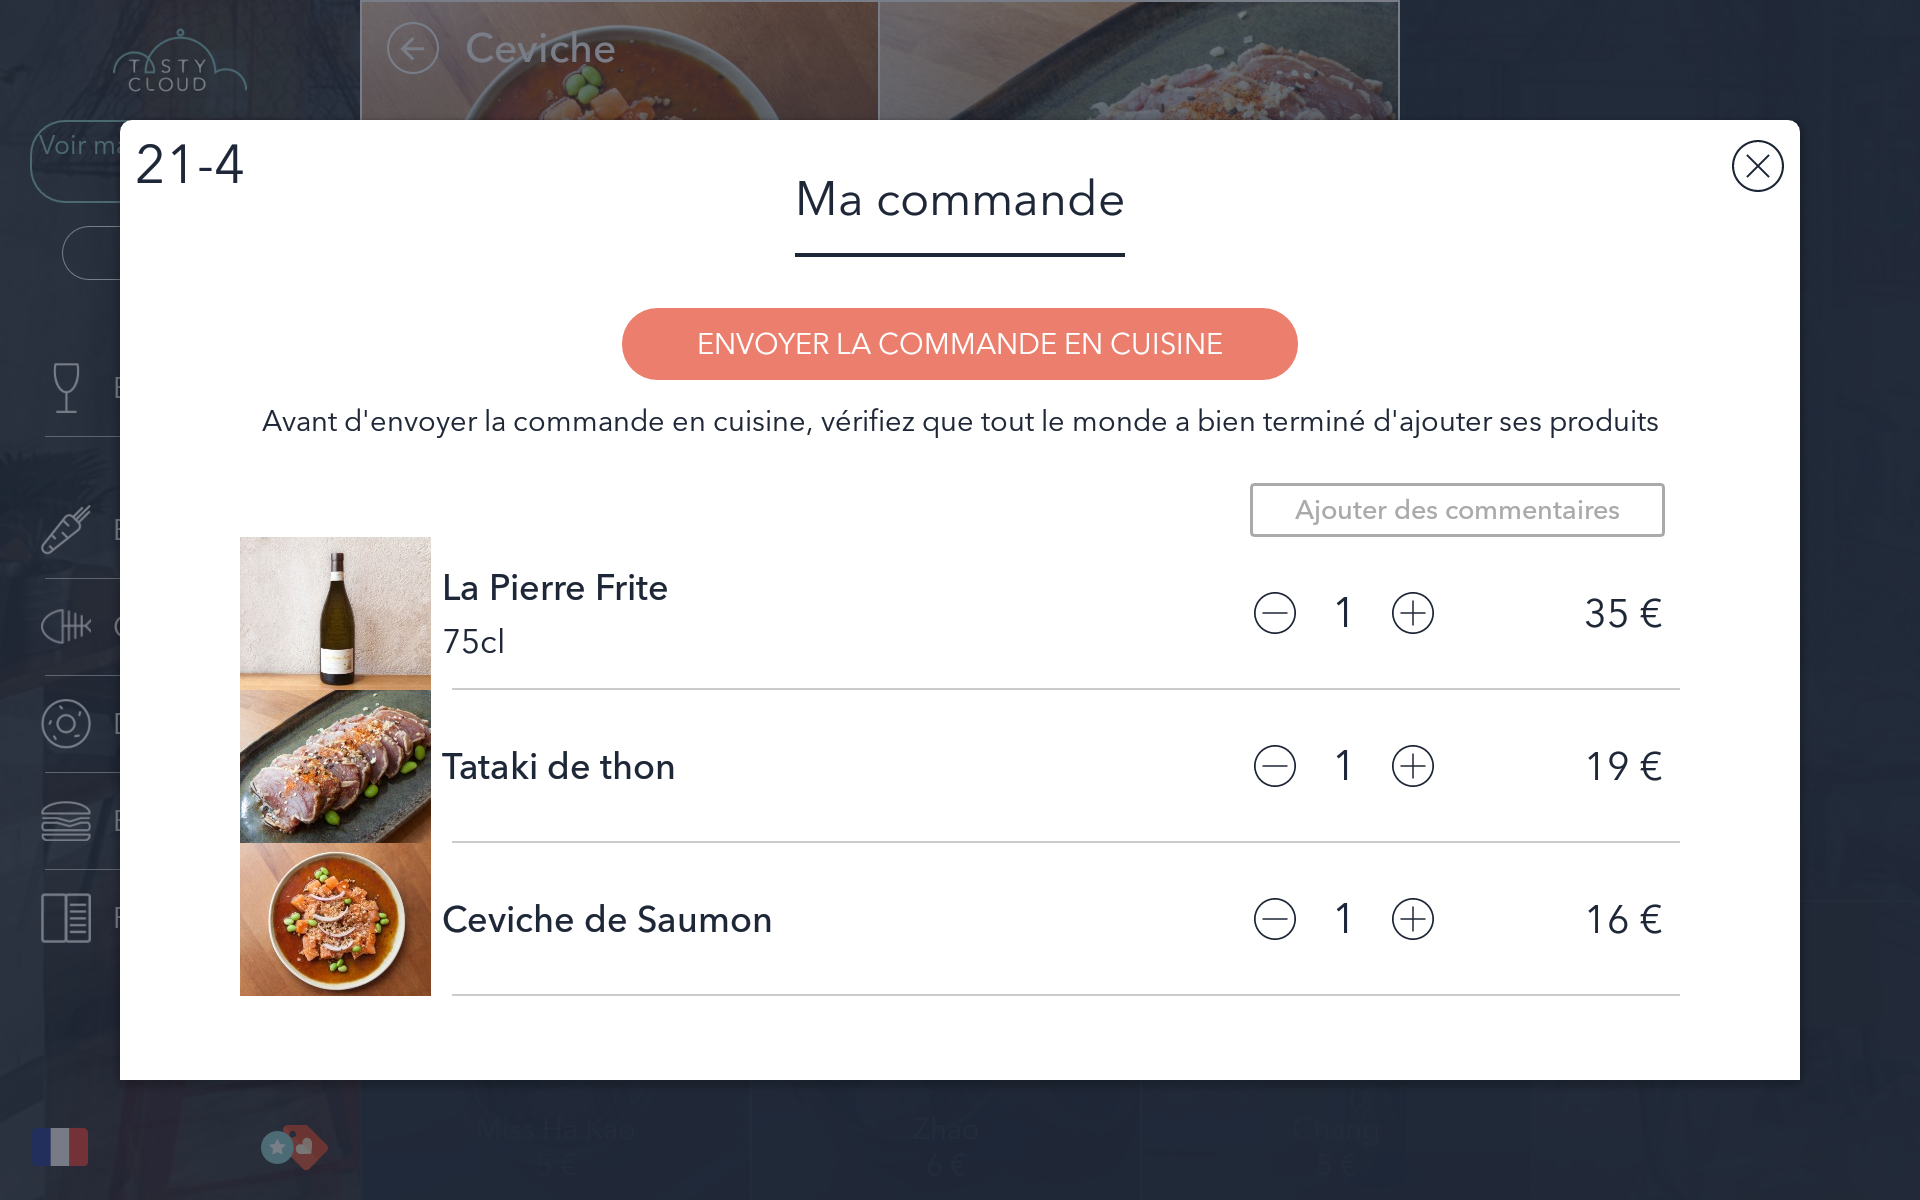
\includegraphics[width=115mm,scale=0.5]{images/divers.png}
  \caption{Le total est caché}
  \label{fig:boat1}
\end{figure}

Dans le menu d'accueil, le restaurateur peut mettre un message de bienvenue pour les clients avec des informations concernant le restaurant. Une demande a été de retirer ces messages (ça et le bouton à propos). Au lieu, cette fois, de mettre une option dans le back office, il a été décidé que dans le cas où le restaurateur décide de ne rien mettre en description et rien dans le bouton à propos, ces derniers ne s'affichent pas. Il a en effet la possibilité d'éditer ces informations dans le back office.

\begin{figure}[!htb]
  \centering
  \begin{minipage}[b]{0.45\textwidth}
    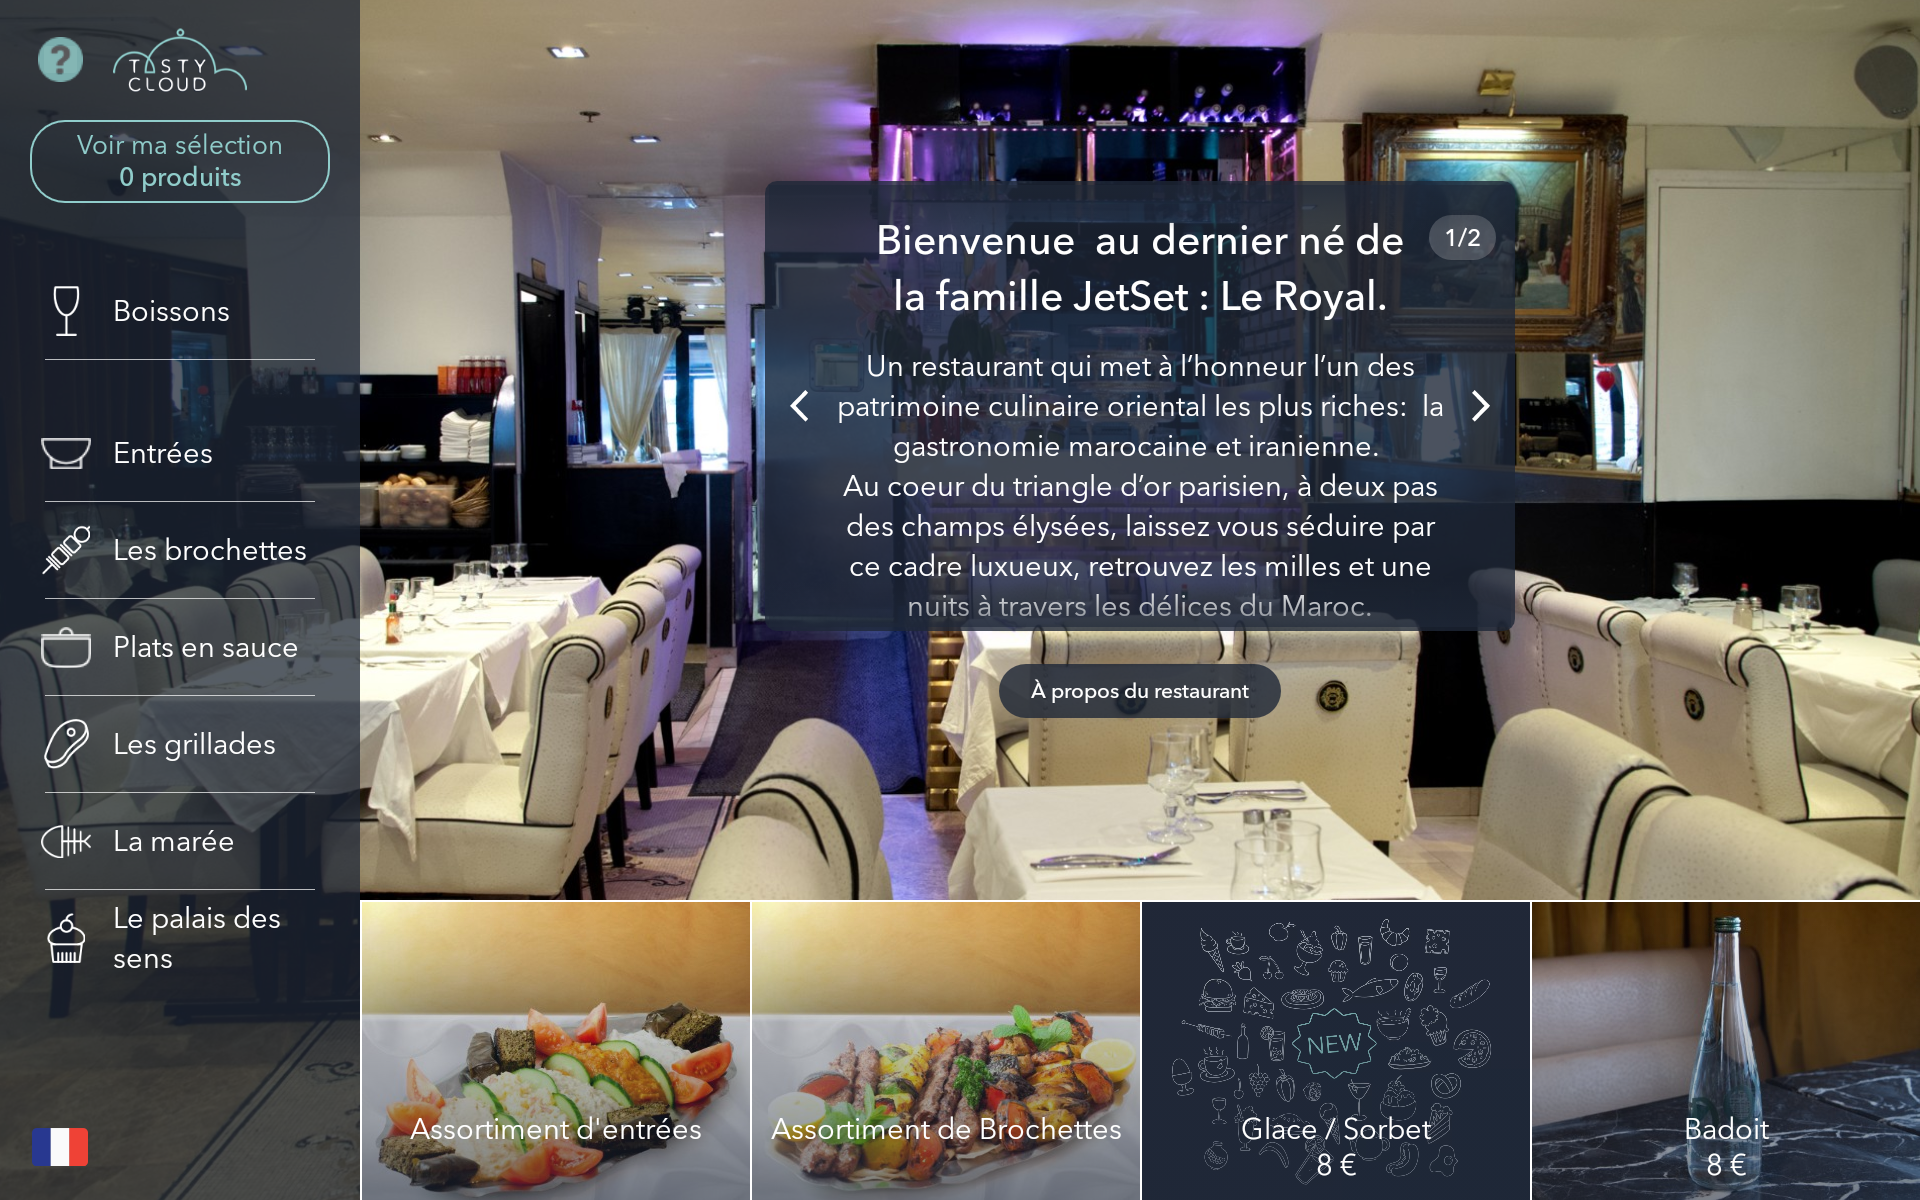
\includegraphics[width=\textwidth]{images/divers2.png}
    \caption{Informations sur l'accueil}
  \end{minipage}
  \hfill
  \begin{minipage}[b]{0.45\textwidth}
    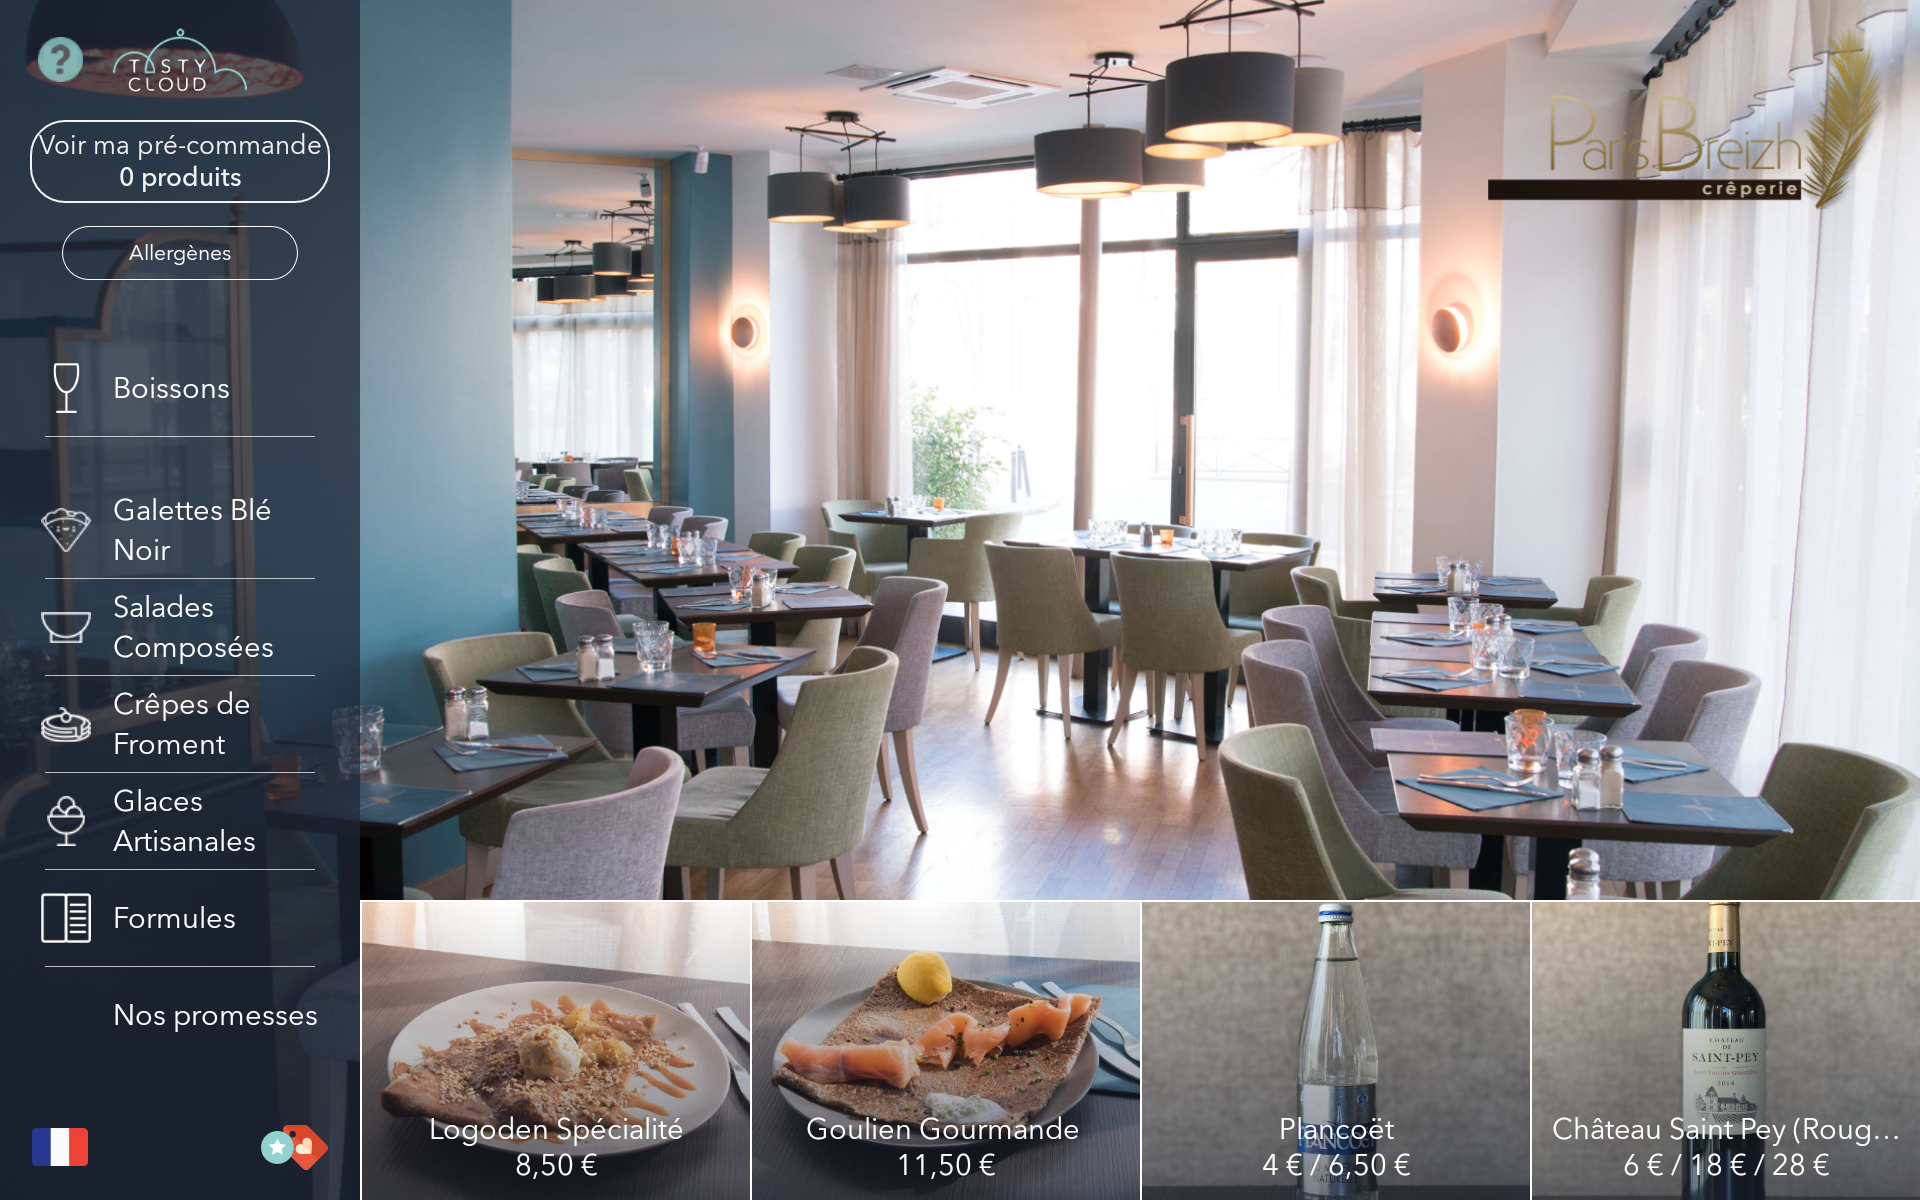
\includegraphics[width=\textwidth]{images/divers3.png}
    \caption{Les informations sont cachées}
  \end{minipage}
\end{figure}

\clearpage

J'ai aussi réglé de nombreux petits bugs qui ont été remontés par des clients ou visibles lors de l'utilisation. Des bugs graphique, en rapport avec la base de données dont même certains qui faisaient crasher l'application. J'ai par exemple géré un cas ou des crashs arrivaient de façon irrégulière sur le changement de restaurant. J'ai fini par trouver le problème en débogage. J'ai refait tout le chemin de changement de restaurant en débogage jusqu'à trouver la cause du crash et pouvoir la régler. Dans ce cas le problème venait d'objets qui n'étaient pas chargés à cause du fait que l'application est asynchrone.

Pour d'autres bugs comme graphique j'ai réglé des détails dans les XML. Ces réglages peuvent être comparables à ce qui par exemple été fait sur le RecyclerView de l'affiliation. Il y a aussi eu des bugs dans le code qui ont engendré des bugs graphique. Par exemple j'ai travaillé sur un cas ou une mauvaise concaténation d'une chaîne de caractères entraînait une répétition du titre. J'ai aussi réglé un cas ou des mauvaises informations apparaissaient dans la sélection avec un chemin d'utilisation bien précis. J'ai aussi travaillé sur des mises à jour rapides. Par exemple sur le fait que les caractéristiques des vins (donc années caractéristiques etc ...) s'affichent si et seulement si nous avons une valeur. Avant l'icône restait même si il n'y avait pas d'informations.

J'ai décidé de ne pas faire de parties pour ces cas car il s'agissait de mises à jour relativement rapides. Par rapport au stage en lui-même, j'ai aussi aidé à la mise à jour sur le site web. Mon travail la dessus se limitait à du HTML et du PHP. J'ai mis à jour des redirections, textes, des pages. Par exemple, j'ai mis à jour certains clients et leur page web sur le site, j'ai fait de même pour la page qui énumère les articles parlant de l'entreprise. Je n'ai pas mis le site directement à jour mais j'ai tout envoyé sur bitbucket et mon tuteur s'est occupé du reste.

\begin{figure}[!htb]
  \centering
  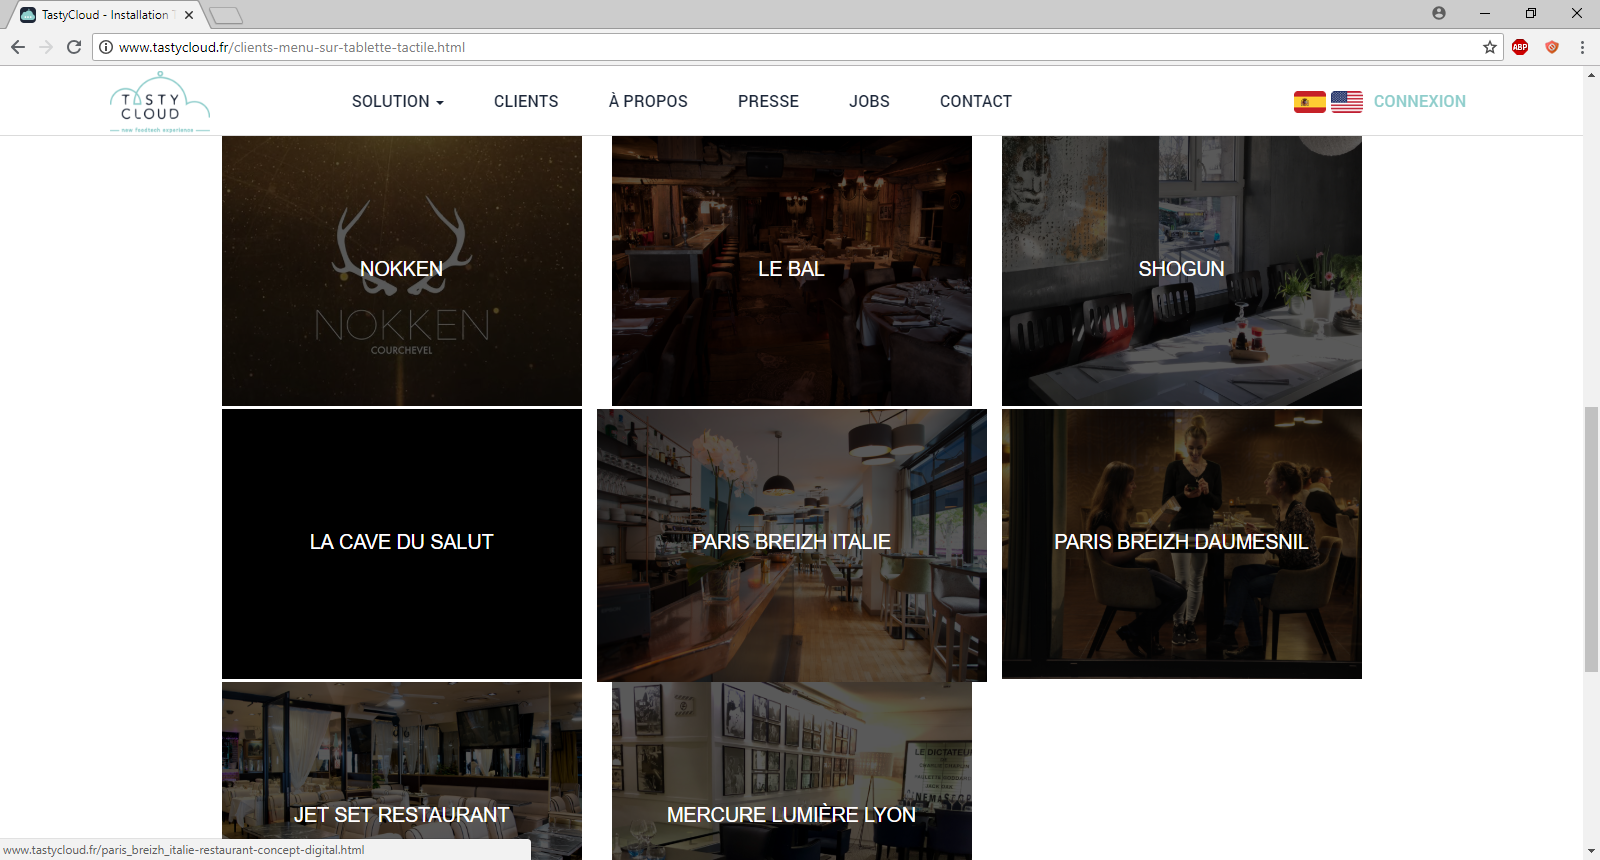
\includegraphics[width=150mm,scale=0.6]{images/site_web_clients.png}
  \caption{Clients ajoutés (du Nokken au Mercure)}
  \label{fig:boat1}
\end{figure}

En plus du travail informatique, j'ai aussi aidé au développement de l'entreprise lorsque l'on mettait en place de nouveaux restaurants. Par exemple l'entreprise a eu un nouveau client avec 50 tablettes en mai et j'ai, avec une collègue, mis toutes les tablettes à jour sur le restaurant. Elles ont ensuite pu être envoyées chez le client. J'ai également mis à jour les photos sur 15 tablettes pour un autre restaurant. Bien que ces travaux n'étaient pas informatiques, ils ont en général toujours été en lien avec les tablettes.

